\begin{fullwidth}
This chapter aims to introduce the concepts and hypotheses used and interrogated in following chapters and is based on a review of the literature. First, a link between properties of the community and the ecosystem services is drawn. Then I examine the use of functional traits to represent plants, plant functioning, and communities. Finally, the impact of intra-specific variability, in particular phenotypic plasticity, on community properties is investigated.

While this thesis is a modelling thesis, it is not a modelling textbook, and rather than an exhaustive description of the different types of models the focus will be placed on selected modelling examples close to the context of this work.
\end{fullwidth}

% #######################################################################################
\chapter{Understanding community dynamics\\and properties: drivers and theories}\label{chapter:coexistence}

% _______________________________________________________________________________________
%\section{The different facets of plant communities: from processes to services}




% _______________________________________________________________________________________
\section{Community assembly and coexistence}

%Community assembly, drivers, interaction and dynamics.


%-----------------------------------------------------------------------------------------
\subsection{Filtering processes: from potential to realised niche}

%\paragraph{Perspectives} % What the fuck do I mean by that?

\paragraph{Plant community}

A community is defined by the ensemble of species that coexist within the same space and time intervals. Communities were first viewed as a group of species that have evolved together to survive within specific conditions. To maintain itself within the community, each species needs to grow during the vegetative phase, survive and reproduce. These steps of the life cycle result from the coordination of multiple physiological processes, supported by the extraction and use of essential resources: light, water, and nutrients. A part of community ecology sees communities as discrete entities with specific characteristics. This view is particularly practical for management as the community type can be associated with certain properties and services, or even particular dynamics and management systems. This view is the base of phytosociology as it is still used. While a discrete approach to community ecology provides practical categorisation, it ignores the fundamental dynamic nature of living systems. In a context of global changes, considering the dynamics of plant communities is crucial to predict how these systems will react to conditions never experienced. Another approach to community ecology considers that communities emerge from the distribution of individuals of a species, the distribution controlled by its genetic and physiologic characteristics and its interactions with other species (Gleason 1926, Whittaker 1975). The distribution of individuals depends on how it is affected by abiotic conditions and interactions with other species or biotic conditions. The joint effects of the abiotic and biotic environment are captured by the concept of the niche \parencite{elton_animal_1971}. While they are many concepts around the niche, the \textemph{niche} of a species is defined by how a species population reacts to abiotic and biotic conditions (resource, competition, predation, survival) and how it impacts its environment. Defining the niche of a species is primarily defining the barriers that constrain the distribution of the individuals of the species.



\paragraph{Abiotic filtering}

The \textemph{abiotic filtering} designates the non-biological variables that prevent the establishment of a species in a habitat. This term generally refers to climatic conditions and resource availability because temperature, water, nutrient and light availability are the main variables that constrain plant development. Other abiotic factors can be considered, such as salinity \parencite{poorter_leaf_2006} or soil properties (pH). These variables determine if a plant (depending on its specific properties) can establish in a given habitat without any biotic interactions. These filters define, for a given habitat, the pool of species (or individuals if genetic variations are considered) that can grow and reproduce in this habitat without interaction. The ensemble of habitats a species can invade if only abiotic factors are considered is called the \textemph{fundamental niche} (see figure \ref{fig:niche}). 

\paragraph{Dispersion filtering}

In addition to this large scale filters, another barrier may prevent a species to invade a habitat: its access. Indeed, dispersion plays a major role in the geographical extent of a distribution area of a species. Dispersion barriers such as mountains, seas or ocean prevent uniformisation of vegetation and reduction of global diversity. Such limits explain the existence of endemic species that grow only in a few locations, despite a larger potential distribution area (as defined by the fundamental niche).

%Based on genetic and physiological properties, plant species may be able to grow and reproduce in different climatic conditions.

%Potential niche

%Abiotic filtering 

\paragraph{Biotic filtering}

Finally, the main factor that can affect the ability of a plant species to establish, is living interactions. For plant species, herbivory and competition are the most important factors, but other forms of interaction can affect the potential niche. The resulting niche, after all filtering processes, is called the \textemph{realised niche}. Competition affects the growth of the focal plant indirectly by reducing the availability of resources, increasing the stress of the plant and reducing its niche (see the interaction between species 1 and 3 in figure \ref{fig:niche}). Competition interactions are major factors shaping vegetation community and are extensively studied both with theoretical \parencite{chesson_general_2000, amarasekare_competitive_2003} and empirical approaches \parencite{kunstler_plant_2016}.

\begin{marginfigure}
    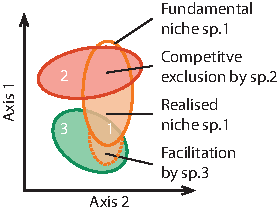
\includegraphics{./1_Introduction/graphics/niches.pdf}
  \caption[Different niches]{The fundamental niche of the \textcolor{myOrange}{focal} species is reduced by competition interaction with \textcolor{myRed}{species 2}, but extended by facilitation interaction with \textcolor{myGreen}{species 3}. This representation of the niche requires the knowledge of the effects of both abiotic factors and all pairwise interactions with other species. A more mechanistic approach of the niche should be considered in IBMs.}
  \label{fig:niche}
\end{marginfigure}

Similarly \textemph{facilitation} interactions also affect indirectly the levels of resources experienced by the focal plant, but in a way that is positive for the focal plant. So they widen the realised niche outside the potential niche (see the interaction between species 1 and 3 in figure \ref{fig:niche}). There are hypothesised to be larger along a stress gradient, where competition interactions are filtered out because they do not allow species maintenance and only positive interactions remain. Such relationships are dependent on the pair of species considered and may change depending on conditions \parencite{callaway_phenotypic_2003}.

\paragraph{Fundamental niche}
 From the point of view of the focal plant, these interactions only exist through the changes in resource availability (even if plants are able to identify their neighbours). In this sense, we can see potential and realised niches as displacements of the fundamental niche (niche defined in term experienced conditions, stresses and resources) within spaces defined by abiotic variables or biotic variables. From this framework, the fundamental niche, or conditions experienced by the focal plant, is the stronger representation of the species niche and the realised niche (abiotic and biotic filters on the niche) emerge from the effects of external factors on this experienced environment.

This point of view should be adopted in models \parencite{berger_competition_2008} because it allows the representation of both abiotic and biotic factors in a shared and generic framework. This is an improvement in comparison to models requiring a matrix of interaction coefficient between species. Such a matrix, in addition to being hard to parametrise, cannot be used in a framework of dynamic strategies as the changing traits would change the interaction\sidenote{A trait-based interaction matrix could be used, but the benefit of the mechanistic approach would be reduced.}. Modelling effort should instead be on explicit temporal and spatial dynamics of resource dynamics. Plant interactions would be captured by the effects of plant functioning (reduction of resource levels in relation to plant growth and resource use) on these dynamics \parencite{berger_competition_2008, morin_comparing_2009}.\\
%Biotic filtering - realised niche.

%Abiotic drivers main thing at global scale... Then interactions and competition.

\textbf{The concept of ecological niche serves as a great tool for theoretical research on coexistence. It encompasses in a convenient way both abiotic and biotic filters of a given species' distribution. While a traditional view of the niche requires considering both abiotic filters and pairwise biotic interactions, fundamental niches and resource dynamics modelling offer an alternative to model realised niches as an emergent property of the model.}



%
%\begin{fullwidth}
%\begin{tcolorbox}[title=The concept of niche]
%
%The ecological niche original refers to the habitat of a species to describe the relationship between a species and the natural environment where it can maintain itself (see \cite{grinnell_niche-relationships_1917} for an early use). This idea allow a finer description of the variables that explain the distribution of a species but is closely related to the idea of range of distribution. It was later refined to better encapsulate the idea of the direct relationship with the biotic environment:
%
%\begin{quote}
%The 'niche' of an animal means its place in the biotic environment, its relations to food and enemies.
%\end{quote}
%from \cite{elton_animal_1971}
%
%The complexity of the requirements for the persistence of a species designated by the term of niche was better captured by the \textemph{Hutchinsonian niche}\parencite{hutchinson_concluding_1957}. It describes the niche a n-dimensional hyper-volume in a space drawn by the environmental variable and resources require to maintain a specific species. This view of the niche allow the development of quantitaive approaches of the niche. Such developments allow the use of statistical tools to link the geographic distribution of species with environmental variables and model the distribution of a species. These species distribution models (SDMs) can be use to study the current distribution of a species or predict the impact of changes in the environmental variables on the realised distribution.
%
%To consider the effect of biotic interactions, the concept of the niche makes the distinction between the fundamental niche where a species can persist indefinetly without competition interactions, and realised niche that result from competition interaction.% This is illustrated in the following figure. 
%% realised and fundamental niches
%
%But this concepts have limitations, and while it takes into account the biotic interactions, the effect of the species of focus on the environment, density related effects or evolutionary constraints are rarely considered \parencite{holt_bringing_2009}. Also, the other species are often treated either as another environmental variable or a competitor \parencite{hutchinson_concluding_1957}. This does not allow to capture complex non transitive dynamics \parencite{levine_beyond_2017} that may emerge from complex and contrasted interaction networks. While being compatible with this representation, context dependent interactions \cite{brooker_facilitation_2008}, can also be neglected in the interacting species are not also considered as an environmental factor. New SDMs approaches include these interactions to better predict the co-occurence on species \cite{pollock_understanding_2014}
%
%% but limitation: other speices effect, but no feedbacks effects: density affect, facilitation, ... new concepts
%% these are better consider into SMD 
%
%% spatial and temporal
%
%% niche and coexistence hteory: realised niche come form the idea of competitve exclusion: explain coexistence iwht niche partitioning, neutrality: niche depends on the variables used to describe it ...
%
%% great conceptual tool: used to described the set of conditions where plants can grow and reproduce
%
%
%
%\end{tcolorbox}
%\end{fullwidth}

%-----------------------------------------------------------------------------------------
\subsection{The complexity of coexistence}\label{subsection:coexistence}

\paragraph{The question of coexistence}
If one wants to better understand and predict dynamics of complex systems, one first needs to understand how such complexity is assembled. Niches can be used to characterise a range of habitats a plant can live in, but because of complex inter-specific interactions, determining the final composition of a community from the list of species that can live in this habitat is not easy. If it is easy to observe diverse ecosystems (from bacteria to plants, insects or algae), it is challenging to determine the processes that 1) group the entities together (in time and space), 2) maintain an apparent stability in the group composition (at least at a certain spatial and temporal scale). 
We can image imagine biotic filtering as a physical filter, the same way the abiotic filter is often illustrated, but this image does not translate the dynamic and complex nature of underlying processes. Biotic filtering emerges as the result of all the interactions between the entities that make it through the other filters. And how these interactions, direct or indirect, play together determines the stability of the diversity \parencite{chesson_mechanisms_2000, levine_importance_2009}.

To predict the outcome of competitive interactions, multiple theories have been developed. Among these theories, we can cite two that have a different perspective on the same question: how do species sharing essential resources coexist in a homogeneous environment?

\citet{chesson_mechanisms_2000} tends to have a population dynamic view of the system and identifies two types of processes that promote coexistence: (1) stabilizing mechanisms, (2) equalizing mechanisms. The former are required to stable coexistence as it a condition of invasibility. In other words, plants can coexist only if one species can invade the other. The condition to such invasion is that the species at low-density grows better than species at high density. This is the case if intra-specific competition is higher than the inter-specific competition. Equalizing mechanisms are processes that diminish the fitness differences between the species, without ensuring stable coexistence. This framework is extended by \citet{adler_niche_2007} in the modern coexistence theory. It states that niche differences \parencite{levine_importance_2009} and fitness differences are the two mains axes of species coexistence. They make the assumption that niche differences define the relative strength of inter-specific versus intra-specific competition. The larger the differences between niches, the thinner is the overlap, and the weaker the inter-specific interactions. Therefore, this can be related to stabilizing mechanisms in \citet{chesson_general_2000}. On the other end, fitness differences also impact coexistence. The lower the differences, the larger are the chances of coexistence. The importance of niche differences required for stable coexistence decreases with the decrease in fitness differences.

On the other hand, Tilman elaborates a theory \parencite{tilman_resource_1982, tilman_plant_1988} around resource use more in line with the idea of fundamental niche expressed in the previous paragraph, the contemporary niche theory. Species are characterised by the impact they have on the resource, and they use the resource for growth. Competition is in favour of the species with the lowest requirement for the resource because competition leads to resource deprivation it can survive. Coexistence is possible if there is more than one limiting resource. In this case, coexistence can be achieved if species have a stronger impact on the resource from which they benefit the most (and intersecting zero net growth isoclines). 


These two theories give strong conditions for stable coexistence, however, they required simplifying hypotheses (all other things being equal, homogeneous environment) that are not met in natural environments. Despite their different approaches, these theories can be united as demonstrated by  \citet{letten_linking_2017} if the impact and benefit coefficients from contemporary niche theory are translated into niche and fitness differences. Despite this unified theory, they applied to a too limited range of situation to be applicable in the context of diverse mountain grasslands.\\
%
%
%
%Focus on interaction: Chesson modern coexistence theory.\\
%
%Chesson vs Tilman. 
%Chesson focuses on interaction and 2 by species, give central idea of stabilizing vs fitness difference.\\
%Tilman focuses more on resources, how the use and impact on resources affect competition and can enable conexistence, but limited coexistence according to this criterion: plankton paradox. No heterogeneity, no temporal dynamics\\
%
%Other things being equal hypothesis (in models at least) does not allow the full diversity to emerge.\


%The plankton paradox in a homogeneous system, where abiotic and dispersion should have a little role in the maintenance of species diversity.\\


%\textbf{One mechanisms alone seems to not be enough to explain fantastic diversity observed in natural ecosystems. However there are multiple theoretical mechanisms that support species diversity and that should take into account in community models: diversity of resources, spatial and temporal variability, frequency dependent effects, etc...}


\textbf{Plant communities require coexistence mechanisms to maintain species richness. Single theories fail to predict high diversity observed in plant communities such as natural mountain grasslands. However, high dimension coexistence processes and complexity seem to be an answer to the biodiversity paradox. In addition to niche based coexistence processes, other mechanisms that promote coexistence must be considered.}




% _______________________________________________________________________________________
 \subsection{Variability and dynamics: driven by the resource}


%-----------------------------------------------------------------------------------------
%\subsection{The complexity of community dynamics} % not very informative title%

Resource dynamics, even with constant resource influx, seems to be the key to understanding plant interactions and dynamics according to \citet{tilman_plant_1988}. Can the resource distribution in time and space explain coexistence?

\paragraph{Community dynamics}

In Tilman's perspective, resources are driven by two things, external influx and internal (to the system) consumption or cycling. The system's structure and composition are responsible for resource dynamics as much as external influx. And these dynamics alter the structure of the community and change the hierarchy within the community. This cycle is well illustrated by the cycles we can observe in forest systems and gap models. Mature forests produce big trees that fall down and create perturbation within the system. The resulting oppening in the canopy enables pioneer species to invade this space without competition. While they grow, other slower species are in shadows and must tolerate this competition, and grow enough to out-compete first established species. Because there is a trade-off between potential growth and shade tolerance allowing this cycle to set up, there is a succession dynamic after each perturbation of the systems. These local events of perturbation support coexistence as a large scale, a coexistence that can be captured by spatially explicit models \parencite{chave_study_1999, falster_plant:_2016}.

\paragraph{Temporal heterogeneity}

\begin{marginfigure}
    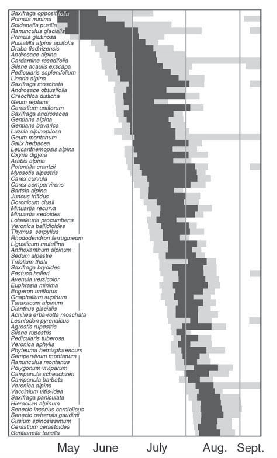
\includegraphics{./1_Introduction/graphics/flowering_m.pdf}
  \caption[Flowering periods of alpine species]{Diversity of flowering periods of alpine species. Evidence of succession in grassland ecosystems. From \citet{korner_alpine_2003}, reproduced with the permission of Springer, license number: 4384850014523.}
  \label{fig:flowering}
\end{marginfigure}

Such drastic dynamics do not exist in mountain grassland communities. But the natural temporal variability of resources due to contrasted seasons also drives diversity in growth strategies. Coexistence comes to the existence of multiple climatic contexts at the same place (but not the same time). As a given species cannot be the most competitive species for all conditions in the whole range of conditions experienced in mountain habitats, there is a succession of species at the top of competition hierarchy \parencite{adler_climate_2006} (see figure \ref{fig:storage_effect} for illustration). The diversity of flowering periods in figure \ref{fig:flowering} is an evidence of this succession dynamics.

\begin{figure}%[tb]
    \classiccaptionstyle
\sidebysidecaption{0.60\textwidth}{0.3\textwidth}{%
    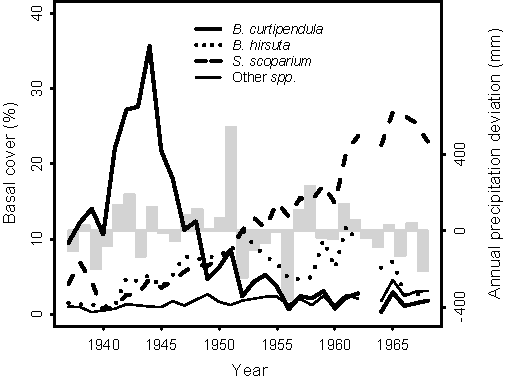
\includegraphics[width=1\linewidth]{./1_Introduction/graphics/succession.pdf}%
}{%
  \caption[Changes in dominance for 3 grassland species]{Changes in observed basal cover for 3 grassland species. This variation in hierarchy illustrates the succession in grassland communities and the storage effect due to the stabilizing effect of climatic variation promoting coexistence. See details in original study by \citet{adler_climate_2006}, reproduced with permission of PNAS, Copyright (2006) National Academy of Sciences.}
  \label{fig:storage_effect}
  }
\end{figure}

This mechanism promoting coexistence because of succession dominance driven by temporal changes in environmental condition is called storage effect \parencite{adler_climate_2006}. The species grow when the conditions match their niche and store the gains to wait until next favourable conditions. This term is generally applied to yearly variations, but the idea can be applied for variations within a growing season, allowing growth and storage until next season.

%
%from Tilman: dynamics of resources
%
%gap model, succession in forest
%
%less structure in grasslands, but also diversity between early and late 
%
%
%
% Succession coexistence and forest models. Dynamics of resources, influx versus impact. Storage effects. Heterogeneity. But how does it link to traits.

%\textbf{From the multiple first attends to explain coexistence with one particular mechanism, scientific community realised that indeed multiple mechanisms are at work to make species diversity in an ecological community. 
%multiple drivers that filter down. + temporal effect (metacommunity, invasion, equilibrium vs long transitions)
 % This multiplicity highlight the need for unifying framework able to cover this diversity of mechanisms and dimensions.}
 
 
\paragraph{Spatial heterogeneity}

The temporal variations have a stabilizing effect on coexistence \parencite{tilman_plant_1984}, but maybe more intuitively, spatial heterogeneity also promotes coexistence. Indeed, spatial variations of conditions at small scale create multiple niches that allow for diversity if measured at a higher scale. This spatial heterogeneity can be overlooked, but in the context of mountain grasslands, where plants are generally small due to high-stress levels and a very fine scale heterogeneity resulting from the terrain texture, it can play as a strong stabilizing mechanism.\\

%
%tilman 1982, spatial
%chesson, 1994, temp, 
%storage effect Adler 2006
%even if stochasticity can reduce coexistence. Fine-scale heterogeneity is rarely taken into account but can play an important role, especially with small individuals.

\textbf{Spatial and temporal heterogeneity play a major role in coexistence maintenance by creating various opportunities or niches, in a given ecosystem. Internal dynamic variation of conditions also support stable coexistence.}

\section{The complexity of diversity}

\paragraph{Larger scale dynamics}

While resource use strategies and resource heterogeneity are important mechanisms for diversity, dispersal processes and meta-community dynamics should also be considered. Grassland communities are not independent of one another, but they are connected by dispersal vectors such as wind and animals. These connections support diversity but not stable coexistence, but remain crucial for community dynamics. Indeed, the link between the community and the meta-community (all connected communities) is a source for a species that may be absent from the focal community \parencite{alexander_plant_2016}. Therefore, in case of transition of environmental conditions, these external species can invade the focal community, accelerating species turn-over compared to a closed community. In the context of global change, it is essential to consider mountain grasslands communities as open systems as the question of invasion by lower altitude species is yet to be solved.

Other larger scale dynamics can impact community dynamics such as species-specific interactions (herbivory or pollination) that lead to dynamic equilibriums. However, modelling such processes are demanding, and while it maintains some diversity, it is not expected to be the main driver of grassland dynamics in the context of global change.

%Role of metacommunity and dispersion dynamics, network effects

\paragraph{Embracing complexity}

Coexistence theory has difficulties explaining high species diversity in communities like freshwater diatoms or mountain grasslands that compete for a limited number of resources in fairly stable conditions. From the previous paragraphs, it seems that these environments are not that stable and that there are numerous mechanisms supporting diversity. Diversity is highly dimensional as it is stated by \citet{clark_resolving_2007}. This complexity, that we just have scratched the surface here, is too high for theoretical models to handle, but constitutes a driving mechanism of community dynamics and a source of species coexistence. Therefore, it is interesting to try to create such levels of diversity \textit{in silico} with a higher level of processes as found in theoretical models.\\
%That does not mean they are not useful, but they cannot consider all these processes at the same time. To study diverse communities, it is required to incorporate at least parts of this diversity in mechanistic models. While it increases the modelling work, model's complexity, and difficulty to analyse results, it allows a stronger representation of communities, of their diversity and enables the identification of main processes, and possible interactions:compensations:synergies between these processes.

%\parencite: coexistence is highly dimensional


 
 % conclusion of the section/chapter:
 \textbf{The evaluation of services relies on a good representation of the plant community and its essential properties. To represent complex interacting systems like vegetation communities, descriptive approaches and theoretical models alone are not sufficient. The main driving processes must be considered and explicitly modelled. Explicit heterogeneity and dynamics of the resources are key to understand and model filtering processes, coexistence mechanisms, and community dynamics. This level of complexity complements the theoretical models and should allow to test the robustness of processes described by these models. However, modelling both community properties and resource dynamics require an understanding of plant functioning and diverse growth strategies. The challenge of community modelling is to keep simplicity in the structure, to integrate the main driving processes and to enable the representation of multiple strategies related to these processes.}
 
 
% #######################################################################################
%\chapter{Considering strategies and functional traits}

\chapter{How to represent plant community}

All plants share the same pool of essential resources and similar physiological processes of assimilation and allocation, however, species differ by their growth rates, niches, and competitive abilities. How do such differences emerge from a common functioning? It seems that these differences can be explained by differences in parameters that characterise this functioning. So considering this diversity is required to represent the diversity observed in mountain grasslands.

 A challenge of modern community ecology is to determine the trajectories the existing ecosystems will follow under new environmental conditions. Species centred approaches, because they are limited to the knowledge of existing response patterns to existing gradients, cannot fully tackle this problem. While the focus shifts toward community approaches, modelling tools should evolve to better answer these newly investigated questions. How can a new representation of plants enable generalisation of the diversity of plant functioning in new conditions?
%Same resources: even more difficult to understand coexistence. Must have differences on how they gather and use these resources. Species is not a handy tool to describe differences in functioning and strategies. A shift in paradigm needed.

% _______________________________________________________________________________________
\section{The continuity of functional ecology}

\subsection{Shift in paradigm: traits and patterns}


%Measure of respiration, assimilation: better insight on the differences between species. A better understanding of plant functioning. Also, show that there is a continuum in plant functioning. This continuum is in line with the observed continuum of community.

\paragraph{A shift needed}

Classical use of niche theory can be observed in Species Distribution Models (SDMs) that link the probability of presence of one species to a multidimensional description of a habitat. The environmental variables are literally used as the dimensions of the Hutchinsonian niche, and directly link the species to its presence in a given environment (see figure \ref{fig:paradigm_shift}, first row). This method is widely used to model environmental niche, but some can also include species interactions to incorporate an explicitly biotic filter. SMDs have good theoretical support and have a lot of practical applications, however, their strength is reduced at the scale of the community where the biotic filtering processes and fine scales dynamics take the advantage over large-scale abiotic filtering. Despite the growing availability of the type of data required to such models, their design does not match the questions relative to transitory dynamics. Community dynamics require fine-scale plant functioning processes to capture the effects of small scales variability and plant interactions, drivers of coexistence. 

This example of modelling approach based on a species centred framework reveals the weaknesses of this framework. The distribution of a species along gradients, or its niche, while it can be captured by abiotic variables, is primarily determined by the fitness components (and whether or not they lead to a positive fitness): growth, survival, reproduction. These variables are not intrinsic properties of species but emerge from the interaction between physiological processes (carbon assimilation by photosynthesis, water absorption, organic matter allocation, etc...) and the environmental conditions. Considering these processes allows to explicit and decompose plant functioning, and therefore could improve the representation of this functioning under new combinations of environmental conditions.

\begin{figure}
    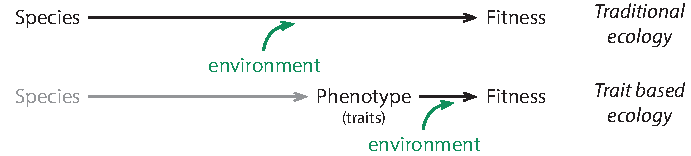
\includegraphics[width=1\linewidth]{./2_PP/Figures/Concepts/species_to_fitness.pdf}
  \caption[From discrete to continuous link between species and fitness]{The shift toward trait-based ecology allows for the decomposition of the link between species and fitness determined by the environment. On one hand, the link between species and traits is better characterised by standardised protocols and the use of databases such as \citet{kattge_try_2011}. On the other hand, the link between phenotypes (defined by trait values) and fitness can be generalised and the role of environment in this relationship better understood.}
  \label{fig:paradigm_shift}
\end{figure}

Most of plant species share the same growth, survival and reproduction processes, but they still differ in these aspects as a function of the abiotic and biotic environment. The solution to shift from species centred paradigm, and its couple habitats-species (or species-environment-abundance like in SDMs), is to explicit the phenotype of these species. By using functional traits to define the phenotype of a species, ecologist can limit the representation effort to the link between traits and fitness physiological properties \parencite{reich_leaf_1992}, and then link species to traits with simpler data collection procedure \parencite{cornelissen_handbook_2003} (see figure \ref{fig:paradigm_shift}, second row).


This shift in paradigm allows for a simpler and functional representation of plant species, that can be later linked to physiological or ecological processes.

%diaz, lavorel, glopnet and try

%this shift worked: falster, 


\paragraph{The rise of functional traits}

The functional traits allow the decomposition of the link between species and fitness, to gain general understanding instead of specific relationships between species, environment, and fitness. However, this decomposition also breaks down the species, that can no more be described by one word, but needs instead multiple quantitative values to be described. The singularity of the species is exchanged for a multiplicity of traits. The link between species and fitness, now broken down by traits, can be analysed in a new light, parts by parts.

This decomposition allows the identification of relationships between morphological traits (easy to measure) and physiological traits (more interesting but harder to measure) \parencite{ackerly_convergence_1999, poorter_leaf_2006,  reich_world-wide_2014}. Response patterns along climatic gradients have also been identified \parencite{niinemets_global-scale_2001} increasing the understanding of the role of the functional traits for the performance of plant species.

This trait-based approach, demanding in data collection effort, benefit from the consistency of the measures \parencite{cornelissen_handbook_2003} allowing pooling of the data into big databases such as TRY \parencite{kattge_try_2011} or Glopnet \parencite{wright_worldwide_2004}. The standardised collection of data all around the globe is a model of centralisation and collection that can lead to major large-scale pattern enhancing the understanding of the functioning of plant communities.

%Requires multiple traits, rise of databases

%Collection of multiple trait sampling.

\paragraph{Are there patterns?}


The use of large data sets unlocks the study of large scale patterns that could be studied before in ecology. For example, \citet{niinemets_global-scale_2001} show strong global patterns along climatic variables for shrubs and trees all over the plant. The mean monthly precipitation of the three driest month and the incidcent daily mean global solar radiation are correlated to leaf structural traits. Such patterns are also observed for leaf structural and chemical traits in \citet{wright_worldwide_2004}.
%some interspecific patterns:

But the functional traits can be used at a more local scale to disentangle the species and the community responses \parencite{kichenin_contrasting_2013, jung_intraspecific_2014}.\\
%along climatic \parencite{niinemets_global-scale_2001, wright_worldwide_2004}
%,on nitrogen (Dwyer)
%
%but also correlations and intra-specific
%change of traits along gradients. Is it interesting?



\textbf{The species-centred ecology has limitations to fully capture the complexity of coexistence and community dynamics processes. The last two decades saw the rise of functional ecology and its ability to capture quantitatively relationships between vegetation and abiotic gradients. The capacity to generalise ecological patterns thanks to easily measurable traits open the door for generalised theories on plant functioning.}

%\subsection{Understanding interaction and competition: a question of symmetry?}
\subsection{Traits and competition}

If traits can describe a species and capture its functioning, it is tempting to consider them to assess competitive interactions. Two visions have been developed to capture relative interactions. As mentioned in paragraph \ref{subsection:coexistence}, trait distance can be a measure of competitive strength. This interpretation is an extension of the hypothesis of the limiting similarity that states that two species with similar niches cannot coexist. If plant functional traits can be used to define the niche, then, trait dissimilarity should be a measure of competitive interaction: the greater the dissimilarity, the lower the interaction. Because the competition is proportional to the absolute distance between traits, the relationship between distance and competition strength is symmetrical. On the other hand, some argue that competition interaction are not all symmetrical, but hierarchical, and that some traits can capture the competition sensitivity and others the competition impact \parencite{kunstler_plant_2016}, therefore the intensity of the competitive interaction is not symmetrical and dependent on the relative trait difference, but rather on the relative strength of impact traits compared to sensitivity traits. It seems that the form of the relationship depends on the type of competition mechanism considered. It will be hierarchical if they compete for the exact same resource (light, water), and symmetrical otherwise (temperature resistance, specific predation avoidance, pollinator, etc...).

Understanding how competition (or any other interaction) is regulated by traits is important to determine competition outcomes with alternative methods than pairwise coefficients that require empirical data to determine. Linking traits and strength of competition interaction would also allow the intra-specific variations to be considered. In this case, determining the exact relationship between trait distance and the competitive effect is crucial as it would change the effect of intra-specific variability (see \citet{hart_how_2016} for example).

But these interactions are not only symmetrical or asymmetrical, there can be non-transitivity promoting dynamic stable coexistence \parencite{levine_beyond_2017}, or be context dependent \parencite{callaway_positive_2002}. Moreover, the nature of the competition relationship (dissimilarity or hierarchy) depends on traits considered \parencite{bennett_reciprocal_2016}. Due to their complexity, interactions cannot be summarised by single trait value comparison but is multi-dimensional \parencite{kraft_plant_2015}. However, traits can inform competitive interaction by informing the plant functioning and the use and effects on the resource.\\

%Functional traits can be used to determine the response of species or communities to abiotic factors, or link morphological traits to physiology. It is also argued that they can capture responses to biotic factors. Traits could be used to 

%CAUTION: do not mistake symmetry of competition (a function of delta traits) with the form of competition (Georges presentation). 


%niches and gradient - symmetric vs hierarchical 

%symetric an asymmetric interaction: it could change the interpretation: identify which traits are in what case.


%\parencite{kraft_functional_2008}
%often need to use multiple traits \parencite{kraft_plant_2015}


%traits used as a proxy for plant interaction and competition. /!\ can be context dependent \parencite{gallaway_2003}.

%but non-transitivity: the key role in maintenance diversity \cite{levine_beyond_2017}.

\textbf{Traits can be a good proxy for competitive interaction but the relationship between trait differences and competition intensity depends on the competition process. If the interaction is transitive, a strong asymmetric pattern can be observed between interaction effects and trait differences, while symmetric interaction reveals niche differentiation processes. Despite these observed relationships, the specificity and multiplicity of trait-mediated interactions promote the use of mechanistic solutions to capture the multi-dimensional and context-dependent nature of plant interactions.}


\textbf{The paradigm shift toward functional ecology allowed the shift from discrete to a continuous representation of species. This change makes easier the representation and study of plant communities, especially along environmental conditions or management gradient. Traits are also used to study plant interactions.  Trait approaches offer a functional link between morphology and physiology that has great potential in generalising environmental effects on the phenotype-fitness relationship. However, the need for multiple traits to capture plant niche differences or similar response patterns of multiple traits suggests underlying structure within trait assemblages. Understanding this structure and how it relates to community dynamics and external drivers is crucial for the representation of diverse communities under changing environments. } 

%Despite the advantages of functional traits, close comparisons and links with theoretical approaches should be used carefully, and underlying assumptions should be interrogated.




% _______________________________________________________________________________________
\section{How trade-offs make strategy space}

%-----------------------------------------------------------------------------------------
\subsection{Trade-offs: capture constraints on species differences}

\paragraph{Leaf Economic Spectrum}
The functional link that is observed between some morphological traits and physiological traits suggests underlying processes that link these traits together. It appears that multiple traits are correlated together at the global scale between species \parencite{reich_evolution_2003,     wright_worldwide_2004, chave_towards_2009, reich_world-wide_2014} and within species \parencite{hu_novel_2015}. This correlation between functional traits of the leaf was described at a global scale by \citet{wright_worldwide_2004}. The \textemph{Leaf Economic Spectrum} (LES), defined by these correlations between multiple traits, draws a continuum of strategies. It spreads from species with high resource acquisition rates and rapid growth rates but low tissue lifespan, to species with longer tissue lifespan but lower growth rates. This is a clear description of a \textemph{trade-off} between strategies, opposing exploitative strategies (high Specific Leaf Area (SLA), high Leaf Nitrogen Content (LNC) and low Leaf LifeSpan (LLS)) to conservative strategies.


\begin{marginfigure}
    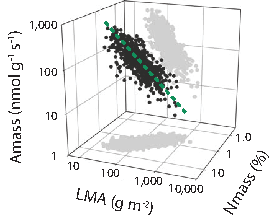
\includegraphics{./Figures/LES1_m.pdf}
  \caption[Leaf Economic Spectrum]{Three dimensions of the LES. Correlation of Leaf Mass Area, assimilation rate per mass unit and nitrogen concentration. This correlation reduces three dimensions (more dimensions not shown) into one axis (\textcolor{myGreen}{- -}). From \citet{wright_worldwide_2004}, reproduced with the permission of Springer, license number: 4384850435840. }
  \label{fg:insurance}
\end{marginfigure}

\paragraph{Strategies}
This axis of differentiation allows ecologists to link quantitative measures to types of strategies that better capture diversity of strategies than discrete typology. These strategies are translated into traits, traits that can be translated into physiological process parameters, then into components of fitness.

In addition to a quantitative measure of species-strategies, such trade-offs simplify a lot trait-based approaches. While many variables can be measured on one individual, correlations between these variables reduce the number of dimensions to consider. This simplification cannot be better illustrated by the work of \citet{diaz_plant_2004} that demonstrate the existence of two major axes of "evolutionary specialisation" that explain a large fraction (41\%) of trait variability: size-related traits, and resource use speed traits. Similar evidence is also found on a global scale in addition to evidence for high levels of coordination between axis \parencite{diaz_global_2016}.


Similar correlations could be found in roots \parencite{ryser_importance_1996, reich_world-wide_2014} but patterns are generally weaker, certainly because of more fragmented data and interactions with micro-organisms that alter the link between morphology and function of roots.

%Where does it come from : Shipley : morphological constraints (as for seed size and seedling growth and survival), hard frontier plus soft frontier (small figure).
\paragraph{Emergence}


\begin{marginfigure}[12pt]
    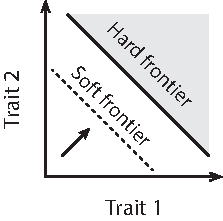
\includegraphics{./Figures/trade_off_emergence_m.pdf}
  \caption[Trade-off emergence]{Emergence of trade-offs between traits because of hard physical-biologivcal frontiers, and "soft frontier" due to selection.}
  \label{fig:trade-off}
\end{marginfigure}

The existence of such trade-off can be explained by constraints that shape the distribution of trait distributions. Trait-function relationships are often depicted as bell-shape with an optimum \parencite{albert_intraspecific_2010}. I rather think that trait and function are linked by monotonous functions, but traits are generally not independent and another monotonous trait-function relationship can constrain the first function. For example, the exchange function of the leaf (and photosynthesis activity), is negatively linked to the thickness of the leave (promoting thin leaves for a higher light capture and photosynthetic activity, but the lifespan and mechanical support of the leaf require denser leaves to be viable. This trade-off in functions, linked by a trade-off in traits (the leaf cannot be both thin and light in one hand, and robust and self-supporting in the other), lead to the emergence of a strong constraint ("hard frontier" in figure \ref{fig:trade-off}) on one side of the relationship, while competition processes out-select combinations of traits that are not relevant on the other side ("hard frontier" in figure \ref{fig:trade-off}).\\


%Diversity of mech: diversity of strategies. more or less independent.\\

\textbf{Trait-based ecology rapidly lead to the observation of trait correlations and trait syndromes between plants. These axes of differentiation emerge from processes that constraint plant strategies. Global characterisations of these constraints should allow a better representation of plant functional diversity.}

%-----------------------------------------------------------------------------------------
\subsection{Strategy-spaces made of trade-offs}

\paragraph{From theory to traits}

Plant diversity is expressed, and visible to anyone, by the variation in shapes and colors, scents and growth forms, but this diversity is the demonstration of a multiplicity of strategies. In an early attempt to make sense of this diversity of strategies, \citet{grime_evidence_1977} theorises the existence of two types of constraints that shape plant communities: perturbations and stress. The perturbation axis captures the variability of community drivers, while the stress axis captures how conditions facilitate or make difficult plant establishment. They draw a two-dimensional space where three regions can be invaded\sidenote{regions of both high stress and high perturbation do not allow establishment}, corresponding to three different strategies: competitive (C) in low stress-low perturbations region, stress tolerant (S) in high stress-low perturbations region, ruderal (R) in low stress-high perturbations region, forming Grime's triangle (\see figure \ref{fig:grime_triangle}).

\begin{marginfigure}
    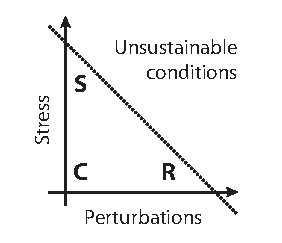
\includegraphics{./Figures/Grime_triangle.pdf}
  \caption[Diversity insurance effect]{Grime's triangle. Competitive (C), stress tolerant (S), and ruderale (R) strategies are dominant in the three regions of the perturbations-stress space.}
  \label{fig:grime_triangle}
\end{marginfigure}

Grime's triangle set the basis for strategy space, and the broad meaning of \textit{stress} and \textit{perturbations} terms allow them to be applied to various conditions. However, the diversity of types of stresses (drought, cold, nutrient availability) and perturbations (predation, fire, avalanches etc...) cannot be specifically captured by such wide concepts. \citet{westoby_leaf-height-seed_1998} highlighted the difficulty to use such space and its incapacity to explain some patterns. According to Westoby, a strategy space\sidenote{called Plant Ecology Strategy Scheme (PESS) in his paper} should: 
\begin{itemize}
\item "express meaningful differences in ecological behaviour between species";
\item allow to "position a plant species from anywhere in the world within";
\item be composed of attributes that "require little enough effort to estimate";
\item make "possible to quantify the extent to which the [strategy-space] captures variation in other plant attributes".
\end{itemize}
Westoby proposes to use functional traits to meet these criteria of functional differences, generalisation, and practicality. Three traits capture the components of Grime's triangle:
\begin{itemize}
\item Specific Leaf Area (denoted L): captures the speed of return of investment of carbon in leaf, as latter highlighted in the LES. High SLA is generally associated with competitive species that capture a lot of light and have a high growth rate. At the other end of the spectrum, low SLA species are more stress tolerant. This axis is the practical equivalent to the axis CS in GRime's triangle.
\item Height at maturity(H): the race to the light, but also captures ruderal axis (time interval between perturbations)
\item Seed mass (S): expresses the capacity of a species to invade recently disturbed environments or the competitive advantage seedlings possess with a larger starting carbon pool. This trade-off between the competitive strength of seedlings against the chance of invading freshly disturbed environment capture well the CR axis of Grime's triangle.
\end{itemize}

The LHS strategy space proposed by Westoby has the advantage to be easily measurable and to allow comparisons between species around the globe \parencite{pierce_allocating_2013}.

\paragraph{Generalisation of strategy spaces}
This approach can be further extended with multiple traits. Indeed, global datasets and databases of functional traits reveal global scale correlations between traits. These correlations, or trade-offs, simplify the representation of plant species \parencite{diaz_global_2016} and translate fundamental axes of strategy differentiation \parencite{reich_world-wide_2014}. Yet, plant communities exhibit extraordinary species and functional diversity suggesting that not all traits are correlated. Trade-offs emerge because of hard (physical, chemical or biological) and soft (competitive pressure) constraints on combinations of functional traits (see figure \ref{fig:trade-off} and \citet{shipley_fundamental_2006}). Therefore, for a given pair of traits, the physical independence of traits and the independence of ecological processes they are involved in should ensure the absence of trade-offs between those. While some traits are related to multiple physiological processes (a composite trait like SLA is involved in water regulation, but also light capture and tissue toughness), traits are often specific to one or two processes.

These trade-offs appear thanks to filtering processes that push the 'soft frontier' toward the 'hard biological frontier' (in figure \ref{fig:trade-off}), and resource echanges in relation with resource availability are such processes. Against climatic filters, plants can either escape (\textit{i.e.} finish a life-cycle before the filtering event) or avoid/resist (develop specific tissues or strategy to pass the filter). This can be observed for drought \parencite{kooyers_evolution_2015} or frost \parencite{korner_alpine_2003}. Resource use strategies and reproductive strategies are also orthogonal \parencite{diaz_global_2016}. 
From this, a generic principle can be formulated stating that the number of observable trade-offs in an ecosystem is close to the number of constraining processes. It is supported by the observation that a limited number of traits (or dimensions, or trade-offs) is often enough to capture the diversity of a vegetation community as in \citet{laughlin_intrinsic_2014}.

The independence of strategic trade-offs justifies that the use of these trade-offs as independent dimensions of a \textemph{strategy space}, defining the diversity of strategies present in a community.

%Same number of strategy axis than filtering processes. (avoidance vs resistance, drought, frost, but could be applied to competition for resources )

\begin{figure}%[tb]
    \classiccaptionstyle
\sidebysidecaption{0.60\textwidth}{0.3\textwidth}{%
    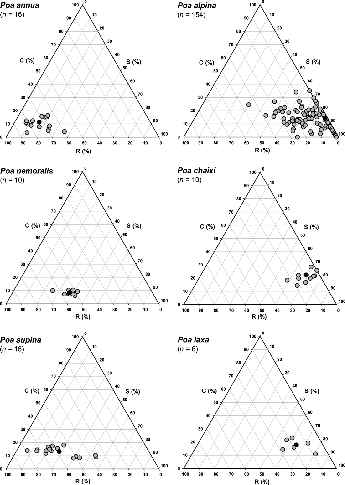
\includegraphics[width=1\linewidth]{./1_Introduction/graphics/CSR_triangle_poa.pdf}%
}{%
  \caption[Empirical evidence for CSR triangle]{Empirical evidence of the CSR triangle in natural communities. The CSR triangle is created by the translation of a multivariate analysis into a coordinate system (see \citet{pierce_allocating_2013} SI for details). "CSR classification of six species of the genus Poa from lowland (left column; P. annua, P. nemoralis, P. supina) and alpine (right column; P. alpina, P. chaixi, P. laxa) northern Italy. Grey circles represent the strategies of individuals, and black circles the mean strategy for the species based on the individuals included in the analysis." from \citet{pierce_allocating_2013}, reproduced with the permission of John Wiley and Sons, license number: 4384950345235.}
  \label{fig:storage_effect}
  }
\end{figure}

\paragraph{Empirical evidence}

The existence of such low dimensional strategy spaces have been observed at large scale \parencite{ pierce_allocating_2013, diaz_global_2016} but also at smaller scales, where the CSR triangle could be identified in ecosystems where precipitation stress and grazing perturbation are shaping the community \parencite{frenette-dussault_functional_2012}.\\

\textbf{The diversity in plant strategies is shaped by the multiplicity of the filtering processes. These strategies are captured in a strategy space drawn by independent trade-offs tightly related to functional traits. These functional trade-offs have great potential in the representation of a functioning plant diversity, while parameter sets allows easy characterisation of species and communities.}



% _______________________________________________________________________________________
\section{How traits link to ecosystem properties}

Now that functional traits, trade-offs and strategy spaces are identified as good candidates to characterise plant functioning and differentiate species, can we link functional traits to \textemph{ecosystem properties} and by extension to ecosystem services.

%-----------------------------------------------------------------------------------------
\subsection{Mass Ratio Hypothesis, Community Weighted Means, and functional identity}

As discussed earlier (chapter \ref{part:introduction}), plant species provide ecosystem services \parencite{mokany_functional_2008}. Some of these services are direct consequences of the characteristics of the species and their functioning. Because of that, \citet{grime_benefits_1998} formulates the \textemph{Mass Ratio Hypothesis} that states: 

\begin{quotation}
... the extent to which a plant species affects ecosystem functions is likely to be closely predictable from its contribution to the total plant biomass. - \citet{grime_benefits_1998}
\end{quotation}

Because functional traits are often continuous quantitative variables, they can be manipulated more easily than categorical variables. Therefore, while phytosociology describes vegetation communities with broad types and approximate abundances, trait-based ecology benefit from this continuity to characterise mean properties of community. The \textemph{Community Weighted Mean} of a functional trait is the average of species-specific trait values weighted by the relative abundance of each species, and corresponds to an extended quantitative application of the mass ratio hypothesis when functional traits are linked to services. These summary variables define the communities in a quantitative way similar to the functional trait for species. In addition to be quantitative, it is functional and responses to disturbing factors can be predicted \parencite{lavorel_predicting_2002}.\\

\textbf{According to the Mass Ratio Hypothesis, some properties of the community directly scale to the characteristics of the most abundant species. In this hypothesis, the \textemph{functional identity}, defined by functional trait values, has more importance than the identity of the species. Community Weighted Mean measures generalise this hypothesis using mean species trait values. While these tools can link community composition to ecosystem properties and services, they require precise measures of plant functional traits to be reliable.}

%-----------------------------------------------------------------------------------------
\subsection{Benefits of diversity}

Certain processes are determined by the most abundant species of a community, but other services and functions may result from the properties of the group. \textemph{Diversity} is the most important property of an ecosystem or a community for a wide audience. This measure is peculiar to groups of organisms and plays a major role in its functioning and the services it provides. Diversity can refer to species richness or functional diversity. The former quantifies the number of species present in a habitat and can take into account the relative abundance of the species. Many indexes can be used to measure this variable representing different perspective or aspect of diversity, such as the evenness, the spatial scale, the functional dimension (see \citet{chalmandrier_communities_2015} for more information).

Functional traits and functional diversity can be used to estimate certain ecosystem services. For example, the diversity of phenology captured in flowering periods (see figure \ref{fig:flowering}) is an indicator of the recreational function of mountain grasslands.
%Empirical studies demonstrate the importance of diversity for multi-dimensional services ... Services are: ......

But diversity also supports indirectly functions and other properties of the system. Multiple mechanisms explain this multiplicity contained in the measure of diversity. 

\begin{marginfigure}
    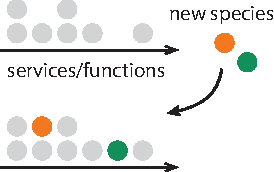
\includegraphics{./Figures/insurance_m.pdf}
  \caption[Diversity insurance effect]{Insurance and selection effects. New species increasing diversity either reinforce existing function (\textcolor{myOrange}{$\bullet$}), or provide new function (\textcolor{myGreen}{$\bullet$})}
  \label{fig:insurance}
\end{marginfigure}


A first importance of species richness is found in the insurance effect that prevents the loss of a function or a service with the loss of a species by ensuring that multiple species provide such function or service (see \textcolor{myOrange}{$\bullet$} species in figure \ref{fig:insurance}). Because insurance effect relies on the redundancy of function, this effect is better captured by species richness than functional diversity. Another way of seeing this notion is the selection effect that states that increasing diversity increases the potential number of services provided by the community (see \textcolor{myGreen}{$\bullet$} species in figure \ref{fig:insurance}), as each species added can provide new function/service (or at worst reinforce already present ones). When the function or service is directly linked to a trait value, this selection effect is directly captured by an increase in functional diversity.

Functional diversity is also associated with ecosystem resilince \parencite{mori_response_2013} and resistence to invasion \parencite{bennett_species_2016}.\\
%benefit of species diversity: insurance effect - portfolio effect ?

%selection, niche complementarity

%what about functional convergence

%productivity 

\textbf{Species richness and functional diversity are often strongly correlated, but they do not capture the same services or effect. Functional diversity is a strong indicator of niche complementarity and its benefits.}

\subsection{Productivity: both community property and ecosystem service}

\textemph{Productivity} of a plant community is mostly sensitive to abiotic conditions, precipitation, nitrogen, and temperature being the main variables influencing productivity. Because of this, there is a large contrast between ecosystems in contrasting environmental conditions (tropical forests and mountain grasslands being two extremes). These differences can be observed in the distribution of functional traits of species, size and resource use related traits being among the most telling ones. 
%Productivity as a marker of abiotic conditions and 
\begin{table2*}
\caption{A comparison of net biomass production (above- plus belowground) in major types of global vegetation, calculated either per year or re-calculated per month of growing season (approximate ranges in brackets). From \citet{korner_alpine_2003}.}\caption{table:productivity}
\begin{tabular}{lccc}
\hline
Biome                                            & Annual NPP & Length of growing& Monthly NPP \\
                                                 & (kgm-2 a-I)                   & season (month)                  & (gm-2 month-1)                 \\ \hline
Humid tropical forest                            & 2.5 (1.8-3.0)                 & 12                       & 210 (150-250)                  \\
Temperate deciduous forest                       & 1.2 (1.0-1.5)                 & 5                        & 240 (110-300)                  \\
Boreal forest                                    & 1.1 (0.3-2.0)                 & 5                        & 210 (60-300)                   \\
Tropical grassland                               & 2.5 (0.2-4.0)                 & 10                       & 250 (70-400)                   \\
Temperate grassland                              & 1.0 (0.2-1.5)                 & 6                        & 170 (70-280)                   \\
Alpine vegetation of  & 0.4 (0.2-0.6)                 & 2                        & 200 (100-300)                  \\
the northern temperate zone & & & \\
\hline
\end{tabular}
\end{table2*}

While community productivity depends heavily on environment properties (climate, soil), it is also dependent on the community, its richness, and the dominant species. The abundance of highly productive species, characterised by high nutrient content, fast-growing and exploitative strategies is responsible for most of a community productivity. Nevertheless, it is hard to disentangle the link between the productivity of the habitat and the productivity of the species living this habitat.

Productivity has another ambiguity: it is both a property of the system and a service. It's a property, and is important in ecosystem services assessment as some services will scale with productivity (\textit{e.g.} carbon storage). But it is also a service, it measures fodder production in grasslands, wood production in forests, etc...\\

%Productivity as a property: depends on the community structure and properties. Leads different services.

%Productivity as a service itself: production (fodder in this case, but OM in forests).

\textbf{Productivity is at the same time a property of the habitat, and the community, and it is a service. While the role of abiotic factors is prominent, the effect of the dominant species and the community structure on productivity should not be ignored. }

%-----------------------------------------------------------------------------------------
\subsection{Trade-offs in ecosystem properties}

Traits can be linked to ecosystem services by a statistical framework \parencite{lavorel_how_2012}. But, in the same way there are trade-offs between traits, the ecosystem services provided by an ecosystem are also constrained. Understanding these trade-offs and the dynamics of the community dynamics allows capture these trade-offs between services bundles \parencite{lamarque_plant_2014}. This link should encourage ecologists to focus on the development of methods to link drivers of ecosystems to community dynamics, to predict changes in ecosystem services (see figure \ref{fig:drivers2services} in chapter \ref{part:introduction}).\\

%lavorel 2012 : trade-off  \parencite{lavorel_how_2012}
%traits - related to trade-off in ES bundles, mostly driven by climate change (rather than management) \parencite{lamarque_plant_2014} limits ?
%\textbf{}


% Section/chapter conclusion
\textbf{ In addition to facilitate the study of the effect of abiotic conditions and biotic interaction, functional traits can be used to describe the community and its main properties to evaluate ecosystem services. Statistical links that can be used to determine these links, and research effort could profitably focus on the dynamics of grasslands communities and the changes in main properties.}

%\textbf{However, the accumulation of trait measurements useful for the study of gradient response patterns and community structure, also reveals the variable nature of traits.}



% _______________________________________________________________________________________
\section{Modelling diverse plant communities}

Modelling mainly consist in deciding what is important considering and worth representing. The choice of how an entity or a mechanism is represented is also part of this decision making. While considering a vegetation community the choice can be on the resources needed, the type of perturbations, or the part of the life cycle you project to be of most importance. For vegetation models that aim for a study of community properties and dynamics, the representation of the interactions of multiple species is key. The strategy-space concept offers a great solution to both the interactions and the diversity of species, while also informing the modellers of the communities' properties.

%-----------------------------------------------------------------------------------------
\subsection{How strategy spaces open vegetation modelling}


\paragraph{The position makes the species}

In a mechanistic model with multiple species, strategy-spaces are simplified ways to define multiple species. A species' identity is fully defined by its position in this space of species-specific parameters. This is a great advantage compared to traditional approaches of vegetation models that rely on strong knowledge about represented species. Because mechanistic models function with shared biological and ecological processes, the differences of behaviours between species emerge not from the functions but from the species-specific parameters. Therefore, to properly model a species' behaviour, in addition to having properly modelled the processes, all species-specific parameters for all species must be determined. This step requires a large investment of time and resources and is proportional to the number of species. Strategy spaces based on trade-offs enable the representation of multiple species, in a constrained and closed trait-space. A greater effort is required to establish such strategy space, as it needs identification of strong trade-offs and the delimitation of ranges along the axes of strategic differentiation. But once established, an infinity of species can populate this robust space without the threat of Darwinian demons. This subject is further discussed in the following chapter (chapter \ref{part:model}, section \ref{chapter:strategy-space}). Because of that strategy space are great tools to consider a diversity of species, when the identity of species is not of primary interest.

While I have no knowledge of living species being projected on a strategy space used in a simulation model, it can be imagined with a projection of measured traits on traits used in the model (even if there can be some discrepancies between the two spaces), in the way of \citet{pierce_allocating_2013}.

\paragraph{In DGVMs}


\textemph{Dynamics Global Vegetation Models} tend to use such strategy spaces to model high diversity with a limited number of traits. A prime exemple of these models is that of \citet{kleidon_global_2000}, and extensions \parencite{reu_role_2011, pavlick_jena_2013}. They use 12 to 15 traits in their strategy space. These traits can be grouped in: allocation traits, tolerance to climatic conditions, resource efficiency, reproduction strategy and tissue turn-over. All these traits are linked to trade-offs in the formulation of the model. A general observation we can make is that these trade-offs often take the form of greater growth or efficiency against greater resistance to stress. This is similar to observed strategies in drought environments \parencite{kooyers_evolution_2015}. These models \parencite{reu_role_2011, pavlick_jena_2013} demonstrate the ability to capture diversity and climatic response patterns, better than plant functional types, with a limited number of traits.


Such approaches are also used to study more specific mechanisms like fire perturbations \parencite{scheiter_next-generation_2013}. In this case, specific traits such as investment in bark and wood density, are included. The adaptive value of the traits is modelled in such frameworks thanks to the inclusion of genetic optimisation processes. This kind of approach is a first step in the understanding of the effect of drivers on community property responses. However, the large scale of these models often does not allow to look at small scales interactions and dynamics, but rather focuses on evolutionary dynamics.


%\begin{landscape}
%
%\begin{table*}%[htbp]
% 
%  \caption[Traits in DGVMs][16 pt]{Tables of functional traits used in Kleidon's family models.}
%    \begin{tabular}{rrrrrr}
%    \toprule
%          & N° & \multicolumn{2}{c}{Authors} & \multicolumn{1}{c}{Cost} & \multicolumn{1}{c}{Benefits} \\
%          &       & \multicolumn{1}{c}{Kleidon \& Mooney - Rue} & \multicolumn{1}{c}{Pavlick} &       &  \\
%    \midrule
%    \multicolumn{1}{l}{Date} &       & \multicolumn{1}{c}{2000 - 2011} & \multicolumn{1}{c}{2013} & \multicolumn{1}{c}{-} & \multicolumn{1}{c}{-} \\
%    \midrule
%    \multicolumn{1}{l}{Traits} & \multicolumn{1}{l}{t1} & \multicolumn{1}{l}{growth response time to moisture} & \multicolumn{1}{l}{\textit{idem}} & \multicolumn{1}{l}{lesss time for C assimilation} & \multicolumn{1}{l}{tolerance to water shortage} \\
%    \multicolumn{1}{l}{} & \multicolumn{1}{l}{t2} & \multicolumn{1}{l}{growth response time to temp.} & \multicolumn{1}{l}{\textit{idem}} & \multicolumn{1}{l}{lesss time for C assimilation} & \multicolumn{1}{l}{tolerance to frost damage} \\
%    \multicolumn{1}{l}{} & \multicolumn{1}{l}{t3} & \multicolumn{1}{l}{seed size} & \multicolumn{1}{l}{\textit{idem}} & \multicolumn{1}{l}{limited dispersion} & \multicolumn{1}{l}{increased seedling survival} \\
%    \multicolumn{1}{l}{} & \multicolumn{1}{l}{t4} & \multicolumn{1}{l}{senescence response time to NPP} & \multicolumn{1}{l}{\textit{idem}} & \multicolumn{1}{l}{lesss time for C assimilation} & \multicolumn{1}{l}{tolerance to climatic variability} \\
%    \multicolumn{1}{l}{} & \multicolumn{1}{l}{t5} & \multicolumn{1}{l}{allocation to reproduction} & \multicolumn{1}{l}{\textit{idem}} & \multicolumn{1}{l}{less growth} & \multicolumn{1}{l}{increased reproduction} \\
%    \multicolumn{1}{l}{} & \multicolumn{1}{l}{t6} & \multicolumn{1}{l}{allocation to AG growth} & \multicolumn{1}{l}{\textit{idem}} & \multicolumn{1}{l}{C expenditure for maintenance} & \multicolumn{1}{l}{increased growth} \\
%    \multicolumn{1}{l}{} & \multicolumn{1}{l}{t7} & \multicolumn{1}{l}{allocation to BG growth} & \multicolumn{1}{l}{\textit{idem}} & \multicolumn{1}{l}{C expenditure for maintenance} & \multicolumn{1}{l}{increased growth} \\
%    \multicolumn{1}{l}{} & \multicolumn{1}{l}{t8} & \multicolumn{1}{l}{allocation to storage} & \multicolumn{1}{l}{\textit{idem}} & \multicolumn{1}{l}{less growth} & \multicolumn{1}{l}{tolerance to C shortage} \\
%    \multicolumn{1}{l}{} & \multicolumn{1}{l}{t9} & \multicolumn{1}{l}{allocation to AG structure} & \multicolumn{1}{l}{\textit{idem}} & \multicolumn{1}{l}{lower PS capacity} & \multicolumn{1}{l}{increased access to light} \\
%    \multicolumn{1}{l}{} & \multicolumn{1}{l}{t10} & \multicolumn{1}{l}{allocation to BG structure} & \multicolumn{1}{l}{\textit{idem}} & \multicolumn{1}{l}{lower water uptake} & \multicolumn{1}{l}{increased access to water} \\
%    \multicolumn{1}{l}{} & \multicolumn{1}{l}{t11} & \multicolumn{1}{l}{relative senescence AG} & \multicolumn{1}{l}{\textit{idem}} & \multicolumn{1}{l}{less growth} & \multicolumn{1}{l}{tolerance to climatic variability} \\
%    \multicolumn{1}{l}{} & \multicolumn{1}{l}{t12} & \multicolumn{1}{l}{LUE regulation} & \multicolumn{1}{l}{\textit{idem}} & \multicolumn{1}{l}{increased respiration} & \multicolumn{1}{l}{increased PS capacity} \\
%    \multicolumn{1}{l}{} & \multicolumn{1}{l}{t13} & \multicolumn{1}{l}{-} & \multicolumn{1}{l}{critical temp. for growth} & \multicolumn{1}{l}{} & \multicolumn{1}{l}{} \\
%    \multicolumn{1}{l}{} & \multicolumn{1}{l}{t14} & \multicolumn{1}{l}{-} & \multicolumn{1}{l}{turn-over of structural pools} & \multicolumn{1}{l}{} & \multicolumn{1}{l}{} \\
%    \multicolumn{1}{l}{} & \multicolumn{1}{l}{t15} & \multicolumn{1}{l}{-} & \multicolumn{1}{l}{turn-over of active pools} & \multicolumn{1}{l}{} & \multicolumn{1}{l}{} \\
%    \bottomrule
%    \end{tabular}%
%  \label{tab:comp_traits}%
%\end{table*}%
%\end{landscape}


\paragraph{In IBMs}

\textemph{Individual-Based Models} are great tools to model community dynamics incorporating local interactions and small-scale dynamics. Because they are interested in smaller systems, IBMs often do not use strategy-spaces and prefer species-specific parametrisation \parencite{soussana_gemini:_2012, taubert_modelling_2014, lohier_analyse_2016}. This is often explained by the focus on heavily managed grasslands with objectives of productivity that need precise predictions and model a limited number of species. But strategy spaces have been used in IBMs to understand diversity patterns in diverse systems such as savannahs \parencite{reineking_environmental_2006} or forest \parencite{falster_plant:_2016}. These approaches successfully describe the diversity and encourage us to use such strategic differentiation spaces.

Higher diversity can be achieved in these models, but numerous species can be discarded. The benefit of a smooth continuum in strategies is that it avoids strong dominance and shifts. Also, the perception of finer changes in the community is possible, while small errors in species parametrisation of species centred models could lead to either no shift (one species dominates and is not sensitive to drivers) or drastic responses (the shift in dominance is abrupt because of no intermediary species). 


%why not too much on IBMs (but Reineking, Marechaud ?, Falster, meh, I guess that Lohier's and Maire's are sorts of strategy space) - because lower community models at this scale: gap to fill.

%But when it's used: break the growth function that links phenotype, genotype and environment ( see figure \ref{fig:paradigm_shift}). Same growth function: no need for specific parameters: same rules for all, but different phenotypes. (the concept of genotype and phenotype would merge for functional traits if there was no other control over other aspects, phenotype defines itself). This is important as it allows for intra-specific variations that would necessitate more complex function in the first paradigm. 

%The growth function, in a simulation model includes all steps from resource gathering and transformation, biomass allocation and phenotype alteration (\textit{e.g.} frost, grazing \textit{etc}...), takes as inputs the phenotype and environment, and gives the new state of the phenotype (and environment). 
%
% figure \ref{fig:paradigm_shift}

%This last paragraph is important to link with the plasticity in a later paragraph.


%-----------------------------------------------------------------------------------------
\subsection{How models inform us on properties and dynamics}

The term \textemph{model} represents a large class of simplified representations of real systems, or conceptual ideas. These are always tools to better understand our world, it can be more by their design and their construction or more by their use (simulations). Here the focus in on simulation models, and particularly agent-based models (of grassland systems). How can these models inform us about real systems?

\paragraph{Hypothesis testing}

One way models can help us understand a system are simulation experiments. This approach is very similar to empirical experiments. The experimenter puts the system, here the model, in different conditions and confronts the results with hypothetical results predicted by theory being tested. In this case, the model is treated as a functional representation of the reality providing the necessary properties to test the hypothesis. And the model shines here in contrast with the real system by its capacity to test a large numer of conditions at very low cost, both in money and time. This is for example the case of the model developed by \citet{taubert_modelling_2014} to test the richness-productivity hypothesis. In the model developed by \citet{droz_model_2013}, the mechanistic properties of the model allow to test the link between the type of interactions and theenvironmental conditoins. These simulation models also allows the prediction/exploration of the system behaviour under alternative climate scenarios \parencite{rodriguez_lingra-cc:_1999, scheiter_impacts_2009}. This is particularly interesting when exploring global change scenarios.

But, this requires a certain level of confidence in the model. This confidence is acquired during the building and calibration process, that both can also give insights on the modelled systems.

\paragraph{Minimal reproduction}

One model, as it is a simplification of a given system, has often a particular perspective, driven by the questions the scientist tries to answer. Because of that, the modeller tries to reproduce only a fraction of the properties/behaviours of the real system. In this case, the models inform us by their capacity to reproduce these essential properties with a minimum number of features and the minimal complexity. This is helpful to identify and understand the core mechanisms that allow the emergence of a particular behaviour of the system. \citet{reineking_environmental_2006} show the capacity of simple allocation trade-offs to let emerge species rich communities, in addition to show the importance of the water (temporal and spatial distribution) as a driver of community structure. The complexity of the studied systems or organism often limits the identification of the causes of a given pattern. Models are valuable when they have the capacity to reproduce these patterns with a minimal complexity, identifying the necessary and sufficient components required for the behaviour to emerge. An example here is the work of \citet{lohier_explaining_2014} on the ontogenetic shift in Root:Shoot ratio for different species.

The calibration process can be necessary to gain confidence in the model, but itself provide new insights. In particular, calibration techniques use data to inform on the value of the model's parameters. These specific parameters can have a value to understand the biology or specificity of the species relatively to other species or the mean behaviour of the model.

\paragraph{On/Off buttons}

A mix of these two forms of insights come from the unique feature of simulation models: their capacity to turn on or off the constituent mechanisms, or rather to switch between different representations of the system. This capacity offers a great flexibility and allows to understand the role of different compartments of the model, and the empirical support for alternative mechanisms. This particular method was used for example in the work of \citet{maire_plasticity_2013} to explore the effects of plasticity on grassland communities.\\

%reineking: the shift in dominance along a gradient
%maire : trade-offs
%
%better understanding of mech. and their effects: \cite{nippert_challenging_2015} root vertical distribution.
%
%reu ?

%schaiter: value of a trait context dependant.

\textbf{The use of strategy spaces in models allows the representation of high diversity in a common plant functioning framework, requiring only a limited number of parameters. Such approaches are very useful to follow the dynamics of communities in a mechanistic framework. Fine-scales IBMs models tend to ignore such simplifications procedure and relies on the direct measure of traits of interest because they generally integrate a limited number of species. IBMs can take advantage of trade-offs and simple strategy spaces to model diverse communities at small scales while keeping biological mechanisms at their core. These models can then be used in different ways to build a better understanding of the modelled systems. However, existing model, based on strategy spaces tend to consider mean individuals and ignore individual variations.}


% #######################################################################################
\chapter{The importance of phenotypic plasticity as a specific case of intra-specific variability}\label{chapter:PP_ISV}

% _______________________________________________________________________________________
\section{Intra-specific variability change the rules}


%-----------------------------------------------------------------------------------------
\subsection{Increasing interest in intra-specific variations}

Trait approaches lead to a better understanding of general patterns of community responses to drivers and of trade-offs in plant functioning. But with the accumulation of large trait databases, the importance of \textemph{intra-specific variability} could not be ignored.

\paragraph{Extend}

The extent of intra-specific variation is a big question as some ecologists point out, because trait-based approaches make sense only if inter-specific differences are greater than intra-specific differences. Consequently the high functional variability within species would weaken theories and generalisation based on mean traits. \citet{violle_return_2012} suggested that the extent of within-population variability relatively to within-community variability should be considered to avoid mistakes in the estimation of coexistence mechanisms. Ignoring intra-specific variability lead to an underestimation of niche overlap, plastic response sto neighbours, or the fraction of resource a species can use. Multiple studies focused on the extent of functional intra-specific variability \parencite{albert_intraspecific_2010, albert_multi-trait_2010} and how to disentangle this variability from species turn-over \parencite{leps_community_2011} in community response. These studies show contrasting results between traits and levels. \citet{albert_multi-trait_2010} demonstrate a within-species variability explaining between 20\% and 40\% of total trait variance, and \citet{siefert_global_2015} note similar levels, but this fraction tends to decrease with increasing community diversity. They also show that the strategic differentiation between exploitative and conservative species is robust to these variations. It appears that not all traits are variable to the same degree and traits like SLA, height, LNC and LDMC are relatively variable while leaf morphology traits variability is lower  \parencite{siefert_global_2015}. 

The variability of multiple traits certainly impacts the functional diversity \parencite{de_bello_quantifying_2011, albert_importance_2012}. All indexes are not sensitive to the same degree, with single trait measure being the most sensitive, but should be used carefully to interpret ecological pattern linked to functional diversity. To overcome this difficulty and disentangle the effects of the different forms of functional diversity, specific indexes have been developed \parencite{de_bello_quantifying_2011}.

The relative extent of intra-specific variability depends on the trait, spatial extent, and species richness, but not on climatic conditions \parencite{siefert_global_2015} suggesting general mechanisms 
%
%\parencite{violle_return_2012}
%ISV is relatively large, ignored in numerous studies, but should not. Viole argue that may alter our capacity to estimate and understand the capacity of species to coexist \cite{jung_intraspecific_2010} suggest to use a hierarchical measure of variance to define the source of variation and that would allow to better explain coexistence mechanisms (niche vs individual variation vs neutral theories)
%
%
%\parencite{siefert_global_2015}
%but intra-specific variation change between traits. Most variable traits being: ...

%\cite{leps_community_2011}

%More interest in trait distribution, variability and diversity. $\rightarrow$ Get to look at intra-specific variability.\\
%\cite{albert_intraspecific_2010}


%\paragraph{}

The fact that some traits are variable, while others are not, implies that some mechanisms structure this variability.
%Intra-specific variability can affect species in multiple ways that are discussed later, 
A way to identify such effects is to look whether variability is structured along environmental gradients, suggesting adaptation mechanisms.

Along such environmental gradients, trait variability for traits like SLA \parencite{poorter_causes_2009} of leaf mass fraction (LMF) \parencite{poorter_biomass_2012} follow similar patterns as inter-specific response \parencite{niinemets_global-scale_2001}, with increasing SLA along precipitation and temperature gradients, and decreasing SLA along radiance gradients (leaf mass fraction shows similar responses). These responses suggest strong constraints (similar to the ones that shape inter-specific differences) shaping this variability. However, species may vary in their response \parencite{kichenin_contrasting_2013}. This contrast can be explained by differences in position around a bell-shaped response curve around the optimum (see \citet{albert_intraspecific_2010} for more details). \citet{kichenin_contrasting_2013} argue this is not the case because alongside a wide altitudinal gradient the response curves observed for any trait or species are not bell-shaped.

This additional level of variability is not always in the same direction as community response driven by turn-over \parencite{albert_intraspecific_2010, kichenin_contrasting_2013, jung_intraspecific_2014} leading to difficulties in predicting the response of the community. These levels need to be disentangled, and in order to do that, mechanisms underlying intra-specific variability have to be understood. This is particularly important because they have multiple effects on how we model community dynamics and understand coexistence mechanisms \parencite{bolnick_why_2011, violle_return_2012}.\\
%
%but if mechanisms are well identified, response patterns not so much.
%
%\parencite{poorter_biomass_2012}
%\parencite{poorter_causes_2009} strong response to light (-), water (+) and temperature decrease (-)
%- suggests selection or plasticity.
%
%\parencite{kichenin_contrasting_2013}
%Jung: not always in the same way \parencite{jung_intraspecific_2014}\\
%\parencite{wellstein_intraspecific_2013} local adaptation, clonal traits
%

\textbf{After the emergence of trait-based ecology and its high potential, the recent focus on intra-specific trait variability questions the strength of mean species approaches. While  intra-specific variability  does not negate numerous conclusions from previous work, because of its large extent and how it alters functional diversity, its effects on community dynamic processes must be interrogated, and underlying mechanisms investigated.}

%-----------------------------------------------------------------------------------------
\subsection{Contrasting effects of intra-specific variations}

Intra-specific variability impacts coexistence mechanisms and community properties in multiple ways. The following paragraphs are not an exhaustive list of all the ways intra-specific variations affect community properties or coexistence mechanisms, but represent a few contrasting examples to emphasise the need for better identification and understanding of underlying mechanisms. 

\paragraph{Jensen inequality}

\citet{hart_how_2016} use a mathematical model to investigate the impact of intra-specific variations on coexistence. They demonstrate the negative effect of intra-specific variations by the intermediate of Jensen inequality effects, that leads to an under-estimation of competitive dominance because of the non-linearity. This certainly can apply to genetic variations. However, intra-specific variability, such as plasticitic responses and local genetic selection, emerges if there are changes or heterogeneity in conditions. These changes, of both traits and environmental conditions, are susceptible to greatly affect the competitive interactions. This conflicts with the assumption of fixed interactions coefficients of such models.

The Jensen's inequality is one of the many mechanism through which the intra-specific variability can impact the dynamics of communities \parencite{bolnick_why_2011}.
%Jensen inequality ... 
%Intra-specific variability can affect 

%Hart: why it is not enough

\paragraph{Niche}

Intra-specific variations (ISVs) can also greatly affect the niche, as any new phenotype is likely to be better adapted to an alternative environment. Therefore, this variability widden the potential niche of the species. In addition to have a potential large impact on the community structure and dynamics, the comparison of the different levels of variance give insights on the driving forces shaping the communities \parencite{violle_return_2012}.

The flexibility offered by a wider niche also impact the mechanisms shaping the community and the relative importance of the habitat filtering and niche differentiation \parencite{jung_intraspecific_2010}, with potential positive impact on the species diversity.
%
%ISV also 
%effect of abiotic filtering
%
%effect on realised niche
%
%neighbours: avoid or increase competition


\paragraph{Contrasting effects}

The previous paragraphs illustrate the contrasted effects the intra-specific variability can have on a community, especially its diversity. Numerous other studies highlight the potential for positive and negative impacts of the intra-specific variability. In additiion to already mentioned studies, the work by \citet{courbaud_intra-specific_2010} highlight that "intra-specific variability allows flexible patterns of community dynamics and could explain discrepancies between observations and classical theories.". More specific work on the phenotypic plasticity, a specific case of ISV, strong effect of this source of variability. It can lead to a shift from competitve interaction to facilitation interactions \parencite{callaway_phenotypic_2003}, or, by impacting the niches, affect negatively the niche separation while at the same time supporting stronger niche differentiation \parencite{roscher_contrasting_2015}. The difficulty to understand and predict the effect of this plasticity is highlighted in the context of the modern theory by the study of \citet{turcotte_phenotypic_2016}. 

Facing this ensemble of contrasted, sometimes conflicting, results, many suggest and support that more work is required to better understand the effect of this variability of the community dynamics \parencite{ bolnick_why_2011, violle_return_2012, valladares_species_2015}, but also try to determine when it should be considered \parencite{albert_when_2011}.\\

%callaway 2003 from competition to facilitation.
%
%\cite{bolnick_why_2011}
%\parencite{hart_how_2016}
%\parencite{courbaud_intra-specific_2010}
%\parencite{turcotte_phenotypic_2016}
%\parencite{roscher_contrasting_2015}
%\parencite{valladares_species_2015}
%\parencite{barabas_effect_2016}
%\parencite{jung_intraspecific_2010}

\textbf{The intra-specific variability has been observed to be an important part of community functional diversity, but also a way the community responds to changes in conditions. In addition to the empirical evidence of this importance, theoretical approaches support contrasting effects of such variations on coexistence mechanisms, evolutionary processes and community responses to climate event or invasion. It is crucial to disentangle different sources of intra-specific variability in order to understand their potential effects on the dynamics and properties of the communities, and ecosystems.}

%-----------------------------------------------------------------------------------------
\subsection{Beyond the mean and the bell-shape: towards more mechanisms in representing intra-specific variability}\label{subsection:bell-shape}

\paragraph{Where is it from?}
Before the increasing interest in ISV during the last decade, this variability was treated as a random effect, partly explaining why it was ignored. But, without discussing too much the philosophy of what is random, we could agree that often the random character of an event is attached to the level of knowledge we have of the conditions leading to this event. That means that intra-specific variability is considered random because we do not have enough information (either too complex, unreachable, or both) do understand/predict the distribution of the different outcomes. But ignoring the mechanisms that lead to this variability causes two simplifications that can alter our interpretations and our understanding of its effects.

First, because it is considered random, ones can overlook the available information about this random event, \textit{i.e.} its distribution. But simply ignoring it, or just apply the same normal normal distribution to all levels of variability. New modelling approaches tend to consider a more precise description of the ISV distribution by looking at its different moments \parencite{dewitt_expanding_2016}(see also \citet{barabas_effect_2016}, to a certain degree). This can lead to errors due to non linearity \parencite{bolnick_why_2011, hart_how_2016}, or non perceived continuous behaviours \parencite{courbaud_intra-specific_2010}.

Second, considering this variability as random, makes you ignore the underlying mechanisms and therefore implicitly formulate a strong hypothesis on the absence of driving mechanism. This can have strong effect on how ones can interpret fundamental theories \parencite{turcotte_phenotypic_2016}. This is somehow similar to the default hypothesis of the competition linked to the distance in the trait-space, that ignore hierarchical competition \parencite{kunstler_plant_2016} or non transitivity \parencite{levine_beyond_2017}. But establishing coherent hypothesis that explain this variability may not be that easy, and is often biased by a "bell-shape" view of the "random" phenomenons leading to hypothesis  that may not explain empirical observations (see the discusion in \citet{kichenin_contrasting_2013} around the hypothesis developed in \citet{albert_intraspecific_2010}).


%There is a difference between how we observe ISV, and why it emerges. What is random? Therefore it is  ... not good ... to apply such simplification of random effect onto theoretical models to predict the effect of intraspecific variability with strong assumptions (observed on the functional trait in wide spatial range, applied to interactions in homogeneous context) on how they translate onto interactions (done in Halt, check Boltnick) 
%\cite{albert_intraspecific_2010} bell shape intra-specific response pattern along gradient, but doesn't stand according to \cite{kichenin_contrasting_2013}. Depends on trait and gradient... cannot assume that, need real quantification. ok if not a gradient response (or gradient is not known).
%Bell shape can emerge from non-measured gradient with linear response. 
%
%Dewitt and Barabas.
%
%The same way the neutral theory is simplifying and brings little understanding to underlying processes and relies on strong hypothesis, considering intra-specificity as a purely random mechanism is insufficient.\\
%Bell shape does not appear in altitude gradient... inconsistencies between theory and empirical data\\
%Strong theoretical hypothesis\\
%refer to asymmetric and symmetric competition\\

\paragraph{Why changing?}

Considering the underlying process of a phenotypic variability is crucial. This is particularly the case for theoretical models that study the coexistence. In such studies, the conditions are often homogeneous, and therefore the fitness or interactions are solely depending on the traits for the given mean conditions. However, under the hypothesis that the variability has an evolutionary value, some sort of variability in conditions is required to see the emergence of phenotypic variability. Either the phenotypes are stable within individuals but diverse for a given species, and this genetic variability provide gain at the level of the population dynamic. Or it the individuals can adapt to contrasted conditions, and the heterogeneity in conditions explain the vairability. In any case, the alternative phenotypes have a better fitness than the phenotype of reference, otherwise these forms of intra-specific variability would have been excluded. Therefore, it suggests that the rules of interaction analysed in these models for the "mean" conditions are not maintained (in term of sign or amplitude) for the specific conditions of the alternative phenotypes. \\

%If most of the changes are plasticity or selection: it changes the effects on interactions and niche.\\
%What are the possible effects? probably it does not affect interaction like \parencite{hart_how_2016} supposes (even if they talk about variations, their conclusions may not be extendable to plastic variations). May change a lot the balance between abiotic filtering and biotic filtering. 
%
%-- go to individual mechanisms, evolution could tackle genetic variations, physiology and ecology on ontogeny, and evolution and ecology on phenotypic plasticity


\textbf{Simple approaches to intra-specific variation constitute an improvement over mean approaches as they highlight processes ignored until now. However such approaches overlook the structure of the variability and underlying processes, leading to simplistic representations and potentially misinterpret the role and effect of this variability.}

% section/chapter conclusion

\textbf{%As ecology shifted from species to traits syndromes, it seems that it needs to go from syndromes to distributions and drivers.
Ecology shifted from species to traits syndromes with great success, but the intra-specific variability constitutes a great challenge for generalisation of observed patterns. By overlooking the processes that structure intra-specific variations, we might lose the capacity to properly interpret the role of variability and refine our understanding of community functioning. The complexity of living communities requires to go further down and consider the individual scale. This is made possible by the accumulation of more and more numerous and detailed data, the emergence of new statistical and simulation tools. The question of the sources and drivers of intra-specific functional variability seems crucial to rise to the challenge it issues.}



% _______________________________________________________________________________________
\section{Phenotypic plasticity: a specific case of intra-specific variability}

Until now, the processes at the origin of intra-specific variability has not been discussed, but to understand how it can alter community properties it is necessary to differentiate the different sources of intra-specific variations as they work in different ways.

%-----------------------------------------------------------------------------------------
\subsection{The different sources of intra-specific variability}

Intra-specific variation can be caused by to two mechanisms: genetic variation and phenotypic plasticity. Genetic variation occurs when individuals from the same species have different genotypes, leading to different phenotypes. On the other hand, phenotypic plasticity implies that the same genotype can lead to different phenotypes. Plasticity can involve epigenetic mechanisms \parencite{
zhang_epigenetic_2013, nicotra_adaptive_2015, beaman_evolution_2016} that blur the frontier between the two forms of intra-specific variability as epigenetic is an inheritable form of plasticity. It is transmitted to descendants but unlike genetic mutation is reversible. To keep thing simple, epigenetic phenomena will not be discussed here.

\begin{marginfigure}[-12pt]
    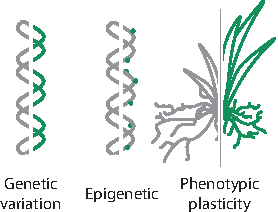
\includegraphics{./1_Introduction/graphics/sources.pdf}
  \caption[Sources of intra-specific variability]{The three main sources of intra-specific phenotypic variability: genetic, epigenetic and phenotypic plasticity. Phenotypic plasticity can involve epigenetic mechanisms.}
  \label{fg:sources}
\end{marginfigure}

Genetic variability (as well as epigenetic) can be detected in case of origin specific response, while if the variability is explained by the treatment, it is a plastic response \parencite{frei_plastic_2014}, and a large fraction of the variability observed in grasslands species is a plastic response rather than genetic variation alone \parencite{frei_plastic_2014, merila_climate_2014}.

\citet{nicotra_plant_2010} provide a good review of plasticity mechanisms and the importance for the adaptation to climate change. They advocate plasticity in functional traits should be considered in mechanistic models as they may play a central role in the speed and adaptiveness of community response to climate change.\\
%Nicotra : pl as an important mechanism for plant to answer to climate change, should look at it.


\textbf{Intra-specific variability can be decomposed in two main types: genetic variability that seems to be closer to random processes envisioned in simple models of intra-specific variability, and phenotypic plasticity that specifically links variations of phenotype to differences in external conditions. These mechanisms of variations are under the control of both evolutionary and molecular processes, that need to be better understood to be disentangled and to better predict their effects on community dynamics.}

%-----------------------------------------------------------------------------------------
\subsection{What is phenotypic plasticity?}

Plasticity is a source of intra-specific variability, but biological processes leading to changes in phenotype can be complex. These paragraphs try to disentangle the different forms of plasticity and the underlying mechanisms.

\begin{fullwidth}
\begin{tcolorbox}[title=Box 1: Molecular basis of phenotypic plasticity] %Toutes les options définies dans le préambule peuvent être définies aussi ici. J’ai juste gardé la possibilité de changer le titre de la box dans ma thèse
The phenotypic plasticity lies both in the perception of external conditions through sensor organ and signalling pathways (auxin pathway for light, root stones for gravity ...), and the integration of this information to alter the development plan. This integration must be coordinated at the scale of the plant according to rules or objectives, question partly explore in this work, but ultimately is applied at the cell levels.\\
\indent Because of the complexity of these pathways and our partial understanding of these mechanisms, we will not attempt to model them. However, I hope that this little overview of molecular mechanisms at the scale of the cell will give the reader an idea of the processes behind the abstract concepts used in this manuscript.\\

The processes of information gathering (through specific organs, cells of organels) and integration of this information finally leading to changes in the phenotype visible at the macro-scale result from similar events at the cell scale. The external signal is captured by a specific receptor at the cell membrane (1), then integrated through phosphorilation cascade (2) leading to numerous alterations of the gene expression sequence (I to IV) because of regulation mechansisms (3 to 8). These regulation mechanisms are diverse, from chromatin changes (3) modifying the accessibility of certain genes, to other gene regulation processes (5 \& 6) or post-transcription regulations (7 \& 8).

\vspace*{0.5cm}

%\begin{figure}

   % \classiccaptionstyle
    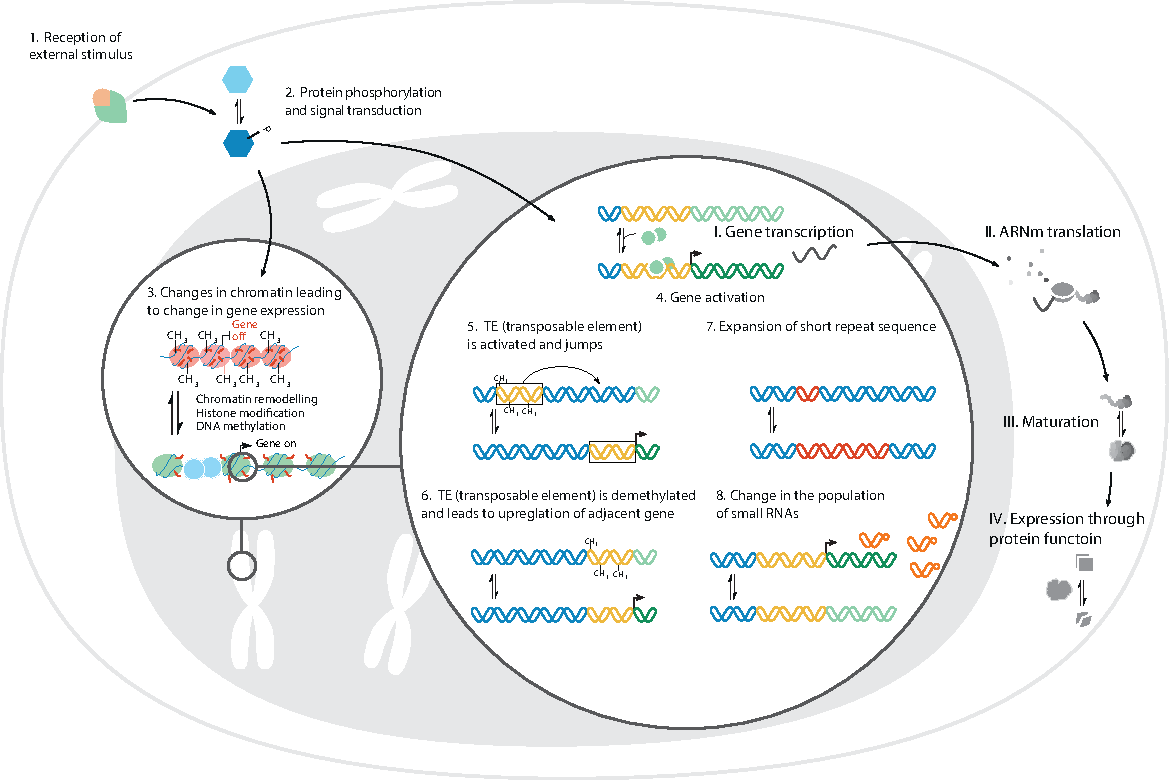
\includegraphics[width=1\linewidth]{./1_Introduction/graphics/molecular_basis.pdf}
  
%   \captionof{figure}{Caption}
{\footnotesize     Phenotypic plasticity is the effect of environment on the link between genotype and phenotype. Plasticity can itself be decomposed in active plastic response that change the internal status of the individual (under genetic control) and passive response that results from the inevitable effect of the environment of the traits on the individual.}
   
   \label{fig:plasticity_form}
%\end{figure}

These regulations of gene expression affect the plant behaviour and development. These regulations are reversible (their effect may not be reversible) but can also be inheritable (\textit{i.e.} 6). The type of regulation depends on the targeted genes, the duration of the regulation, and other factors. This multiplicity of regulatory processes at the scale of cells, in addition to the interconnectivity of genes, signalling pathways and tissues interactions, demonstrate an extraordinary potential for the regulation of both functioning and phenotype of plants. Therefore it seems that the molecular basis does not limit the plasticity, but it is rather the difficulty to anticipate the future and to define the best strategies that limits the benefits of phenotypic plasticity.

The diversity of mechanisms and scales (both spatial and temporal) these processes can act inside of plant gives an idea of the diversity of strategies a plant can deploy to face changes in its environment. Considering this complexity, only a small fraction can be explored in such model as \model, but hopefully, it will help make progress in our understanding of the role of these molecular mechanisms at the scale of the community.
\end{tcolorbox}
\end{fullwidth}






\paragraph{Forms of plasticity}
Phenotypic plasticity is the capacity of a species to produce individuals with the same genotype but different phenotypes. This difference in phenotype should be an active process, not the results of direct alteration of the phenotype by external factors without changes in internal functioning. This change in internal functioning process has the objective \sidenote{in the sense it has been selected because it provides this capacity} to match the phenotype with expected future conditions to maximise the individual fitness. The expression "expected future conditions" is key here, as it is this projection that drives the plasticity.
%Confusion, phenotypic plasticity is a particular phenomenon, driven ...\\

\textit{Active plasticity is used for predominantly anticipatory, and often highly integrated, phenotypic changes in response to some environmental cue or signal, and reflect modifications of developmental pathways and regulatory genes.} Forsman - 2014\\


Passive plasticity, on the other hand, may stem from direct environmental influences on chemical, physiological and developmental processes, and is generally not considered anticipatory, but a mere consequence of the environment, such as stunted growth owing to low resource levels.\\


\begin{figure}
    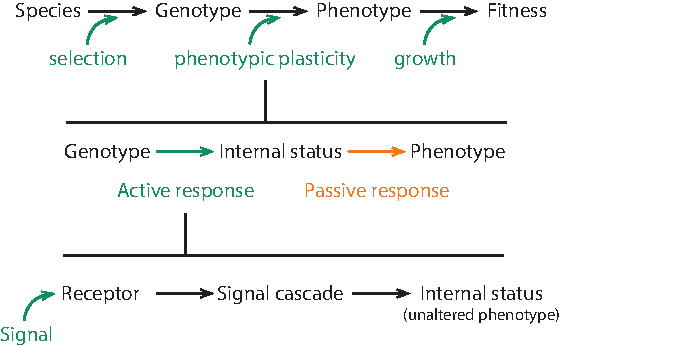
\includegraphics[width=1\linewidth]{./2_PP/Figures/Concepts/genotype_to_phenotype.pdf}
  \caption[Decomposition of plastic response]{Decomposition of phenotypic plasticity as a step between the genotype and the fitness. Phenotypic plasticity is the effect of environment on the link between genotype and phenotype. Plasticity can itself be decomposed in active plastic response that change the internal status of the individual (under genetic control) and passive response that results from the inevitable effect of the environment of the traits on the individual.}
  \label{fig:plasticity_form}
\end{figure}

%\paragraph{Biological process}
% The details of the molecular changes that occur in a plastic response ). 
Active and passive plastic response can be discriminated by the position of the control: internal for the active plasticity, or external for the passive response. In the case of active plastic response, the signal from environment must be integrated (from physical or chemical to information) then transferred to response organs. These organs respond to the integrated signal by changes in their expression levels (\textit{internal status} in figure \ref{fig:plasticity_form}) as summarised in figure \ref{fig:active_plasticity}.

Changes in phenotypes are controlled mainly by changes complex development processes. These processes involve numerous proteins and signaling pathways. Genes expression of proteins (transcription factors, enzymes, signalling proteins...) is controlled by specific mechanisms with various degrees of speed and duration (instantaneous regulation response, to inherited epigenetic adaptation). Some of these molecular processes are detailed in box 1 above in relationship with gene expression pathway (see also \citet{nicotra_plant_2010}).\\


\begin{marginfigure}[-24pt]
    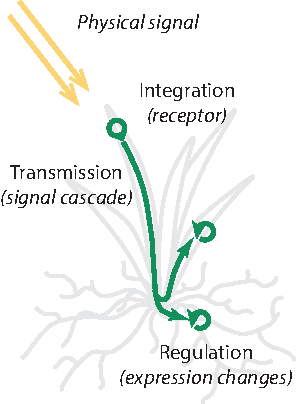
\includegraphics[width=1\linewidth]{./Figures/active_plasticity_m.pdf}
  \caption[Active plasticity]{Mechanism of active plasticity. Integration of a physical (or chemical) signal, transmission and regulation of phenotype through regulation of gene expression, or post-transcription regulations.}
  \label{fig:active_plasticity}
\end{marginfigure}

\textbf{Active phenotypic plasticity is an integrative process at the scale of the individual that aims for an improvement of plant fitness by the adjustment of its morphology according to environmental cues. It often relies on multiple regulation processes. Modelling the extent and the rules of such mechanism is not an easy task that might depend on the context and the framework used.}

%-----------------------------------------------------------------------------------------
\subsection{How to model phenotypic plasticity}

A plastic response can involve numerous genes interaction in networks of regulatory pathways. The objective of an ecological model is not to reproduce this complexity, but the basic behaviours emerging from this biological complexity\sidenote{this biological complexity can be explained by the simplicity and a limited number of basic biological units living organism are made of, and the emergence through a simple mutation-selection operation. This complexity can be mimic by simpler and freer mathematical design.}. The basic components of the active plastic response are the perception of the external signal, its integration into meaningful information and the transformation into phenotype modification.

\paragraph{Reference and plastic traits}

%Modelling is a compromise, a balance must be found between precision and consistency, between complexity and simplicity. This means that not all facets of a plant can be modelled, and simplifications must be adapted to have an efficient representation of a plant. The level o precision is defined by many aspects, but mostly the questions the modeller want to answer, and the main processes that drive the interrogated phenomenon. In any case, the plant is represented by variables, that can be traits in ecology, that correspond to aggregates of a plant true characteristics. \cite{lucas_plant_2011} 
Every growth model is plastic. Every growth model predicts different phenotypes for plants sharing the same phenotype (often just defined by the species affiliation) growing in different conditions. But most of this plasticity is passive, and it could be encompassed in this personal definition of the notion of \textemph{growth function} (see figure \ref{fig:plastic_function}). However, among vegetation models only some of them claim to include phenotypic plasticity \parencite{maire_plasticity_2013}. What criterion can be used to distinguish active from passive plasticity in the context of plant modelling?

The use of information from the environment to change the phenotype in order to have a better fitness is active plasticity see \citet{forsman_rethinking_2014} for a discussion of the form of plasticity). But in practice (in models)\parencite{maire_plasticity_2013}, often nothing really separates the two as plasticity is often modelled as a general mechanism shared by all species (but see \citet{jablonka_adaptive_1995} for discrete strategies in clonal plants) and local environmental variables are used to determine the phenotype of a plant in both cases. Only the justifications and the forms of the linking functions are different, and they may involve different traits. This idea is illustrated in figure \ref{fig:plastic_function}, where the phenotype is first defined by the genotype then controlled by the growth function as a function of current phenotype and environment (see figure \ref{fig:plastic_function}, left column). There are no differences between plasticity of two species if two species have the same phenotype, then in a similar environment, they would express the same plastic response (middle column). I argue that plasticity, to be considered as an active process, should be under a genetic control (\textit{i.e.} species-specific parameter). This means that, despite a shared rule and similar phenotypes, the plastic would be different and would depend on a species-specific parameter (right column). Phenotypic plasticity should be a form of \textemph{strategic plasticity} to be analysed differently from a growth function.


\begin{figure}
    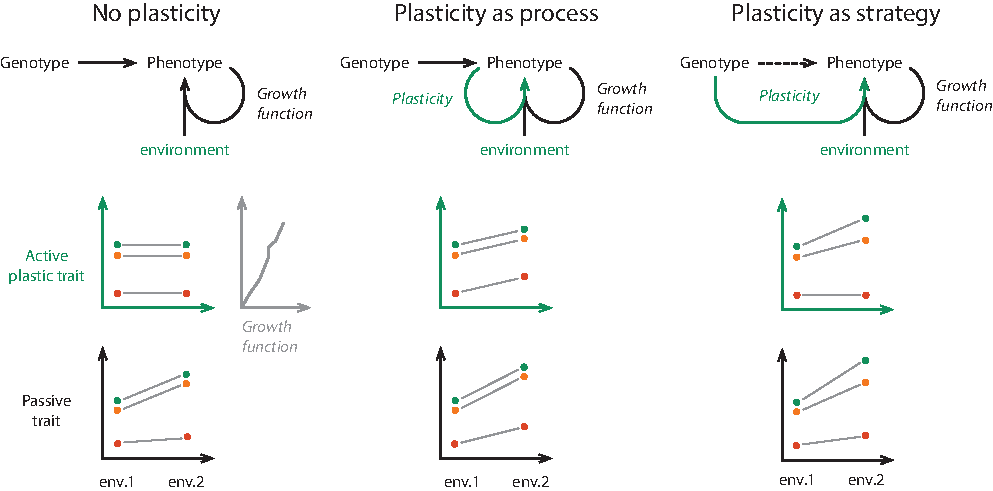
\includegraphics[width=1\linewidth]{./1_Introduction/graphics/plastic_function.pdf}
  \caption[Forms of plasticity in models]{Three forms of plasticity in models. \textit{No plasticity}, the differences in trait (passive trait such as total biomass) are explained by the growth function. \textit{Plasticity as a process}, the active plastic traits change in the same way in both condition: the process is not just growth, but it is shared between all species. \textit{Plasticity as strategy}, the species respond in different ways despite sharing the same starting phenotype and environments. The plasticity is a strategy determined by a genetic trait.}
  \label{fig:plastic_function}
\end{figure}

Only the plasticity as a strategy differentiates conceptually the plastic response with the growth response. Paradoxicaly, this difference is better embodied in models with reaction norms (that generally differ between species), than mechanistic models that share a same mechanisms for all plastic responses. Plasticity as a strategy is possible within models with a shared plastic response mechanism, but they require additional species specific parameters to control this plastic response. This is because these models \parencite{lohier_explaining_2014} are based on the assumption that the general plant functioning can be captured by shared processes and the differences are captured between the species-specific parameters. So, it is logic in this context, if we consider the plasticity as a process different from the "growth function" only, to attribute species-specific parameters that control the plastic response. The adaptive value of this traits, and therefore of the plasticity, can now be dependent on the other traits, and the plasticity can be exposed to mutation and selection processes. While this a mid to long-term objective, it is first important to define strong plasticity mechanisms.

%
%Moreover, no integration function, 
%
%Two questions emerge from this: if growth function and plastic response are different (conceptually), how to determine each of these functions?
%How the genetic control affect the phenotypic response? Or why would it be beneficial to have multiple rules - non-discrete perspective on plasticity?

%However, the linking function used have different justifications and forms, and acts on potentially different traits. In order to mimic active plasticity observed in nature the environmental variables should be integrated by plants, however, this integration function is often ignored \cite{maire_plasticity_2013}. Therefore plasticity is mostly framed by the traits that are affected by the 


%One definition could be \textit{any variation of traits that alter plant functioning}, but that would not be enough as grazing modification of  ... information to change traits ... hum OK, but mostly just a change in frame of reference. Still, affect the niche.


%every model plastic, but mostly passive

%we want active plasticity, what's distinguish plasticity types is not the frame of reference, but the strategy: it's a choice: determine by another trait that characterises the response.
%
%what makes it plastic: find the invariance. Laughlin? (what's invariance anyway)

\paragraph{Plasticity rules: a question of drivers}

As mentioned, the plasticity needs a \textemph{drivring rule}. In a physiological perspective, it a set of signalling cascades triggered by external stimuli. In an evolutionary perspective, it would be a sort of optimisation function. It is the work of the modeller to translate the shaping effect of the evolutionary forces, into responses that can be coded into chemical reactions and make sense in the context of the model (a plant can create an estimation of future condition, but cannot determine precisely these conditions). From this, ones can have a more practical approach, and mimic the chemical cascades, and their effects of the physiology and morphology of the plant. The \textemph{reaction norm}, that determine the new target phenotype as a mathematical function of an explicit external variable (\textit{e.g.} the leaf thickness as response of the received light energy \parencite{feller_mathematical_2015}) is a good example of such approaches. But there are an infinity of functions, and the shape and the parameters of these functions, the rules, are extracted from the empirical knowledge, data or from a theory. In this case the plasticity is defined by a set of rules, linking one variable with one particular traits.

But our understanding of plant physiology et ecology can also help us modelling plasticity with a more conceptual approach. The evolutionary objectives can be translated in general rules, under the assumption that the biology and chemistry of plant allow the coding of these rules. This could be seen as finalist, but make sense in an evolutionary perspective. The plant try to respect the established rules by modifying all the plastic traits. In this case, all traits follow an explicit general objective, such as the functional equilibrium \parencite{hirose_vegetative_1987, lohier_explaining_2014} or a net return optimisation \parencite{mcmurtrie_leaf-trait_2011}. In this case, the link between the phenotype and the objective must be clearly establish in order to determine what is the best phenotype.

Defining the rules driving plasticity is a complex task. It requires to consider the plastic dimensions (traits), the available information of the external conditions (external sources of stress) and the general objective. Moreover, there is an apparent contradiction between the idea of a driving rule and the plasticity as a strategy. If the the plasticity is driven by a general rule given by strong evolutionary principles, how can species express diversity in plasticity? To have different strategies, plant can follow this general rule to a different extend, with strong plastic response and weak or null responses. This could be seen as a "trust level" in the general driving rule. Alternatively, multiple rules could compete in a same model, the species parameter determining the rule to follow would be the plastic strategy mentioned in the previous paragraph. Using a general principle to drive plasticity has the advantage to integrate all plastic responses (from root to shoot, from anatomy to physiology) in a coherent framework, and avoid incoherent responses. But these incoherent responses can a be a form of limit of the plasticity \parencite{dewitt_costs_1998, van_kleunen_constraints_2005}, maladaptive responses that are observed in nature. Maladaptive plasticity could still emerge from such model, because if the response are coordinated and coherent, the estimation of conditions determining the best phenotype main not be good one.

In any case, the drivers of plasticity, reaction norms or general rule, must be determined as a function of the traits of interest and the context of the scientific questions examined.\\


\textbf{The phenotypic plasticity differ from other form of intra-specific variability by a strong and direct control of the changes in phenotype by the plant, in relation with the experienced external conditions. Such level of control can only be model by precise rules that tight the forcing variables with the response traits in a coherent framework, based on both physiological and evolutionary principles.}

\textbf{ Modelling phenotypic plasticity as a strategy of the species requires both a framework link forcing variables and traits, and authorising differences between species. While many options are available to model this phenomenon, the choices of the modeller should be driven by the specificity of the system and the scientific question.}
% _______________________________________________________________________________________
\section{Toward an integrative framework of plant strategy and phenotypic plasticity}

Adaptive plasticity in models is often a layer on top of the species strategy, it acts more like a new mechanism, rather than a strategy within the already existing growth process. To interrogate the plasticity as a dimension of plant growth and an evolutionary process \parencite{bradshaw_evolutionary_1965} (see also work of Scheiner \parencite{scheiner_genetics_1989, scheiner_genetics_2002, scheiner_genetics_2012}), or better understand the cost and limits of plasticity \parencite{dewitt_costs_1998, callahan_phenotypic_2008, auld_re-evaluating_2009}, or the effect of plasticity on coexistence and community dynamics \parencite{hart_how_2016}, plant strategies and plasticity need to be blended together in an integrative framework.
%For models we talk about plastic models versus models that do not include plasticity. It makes sense to differentiate models based on the inclusion or not of plasticity, but if the plasticity is considered an important mechanism for the system, then we need to consider what's plastic and what's not. Traits 

\subsection{Plastic strategies}

Resource-use and allocation strategies have been related to environmental conditions in both empirical \parencite{wright_leaves_2002, ackerly_functional_2004, poorter_leaf_2006}, conceptual \parencite{grime_evidence_1977, westoby_leaf-height-seed_1998} and modelling\parencite{kleidon_global_2000, scheiter_impacts_2009, reineking_environmental_2006} studies. Moreover, functional traits show evidence of intra-specific changes along environmental gradient \parencite{kichenin_contrasting_2013} and intra-specific economic spectrum \parencite{hu_novel_2015}, and constraints that shape main ecological trade-offs are certain to also constrain individual traits. Therefore, if strategies vary between and within species along environmental gradients, it makes sense to imagine that plasticity as changes in strategic traits. This goes beyond changes in spatial allocation\parencite{schapendonk_lingra_1998}, or parameters not identified as strategic traits \parencite{lohier_explaining_2014, feller_mathematical_2015}. Considering strategic traits is not common practice because it blurs the limits between species that are not well identified by these traits any more\sidenote{especially when a relatively low number of species-specific traits are considered}.

%Unlike the conception of plasticity in models \cite{ maire_plasticity_2013, lohier_explaining_2014}. Why? because blur the frontier between species, species-specific traits are not that specific anymore. But remember "species about trait than trait about species 
However, while this interpretation makes sense, the species and the individuals do not have the same constraints, and plasticity cannot be as large as intra-specific diversity as there are limitations to plastic development \parencite{dewitt_costs_1998, auld_re-evaluating_2009}. Moreover, it seems that rules that drive plastic may not be the same as the ones that drive intra-specific genetic variations  and inter-specific differences\parencite{ryser_consequences_2000}, explaining contrasting response along gradient or between experimental drought treatment \parencite{kichenin_contrasting_2013, jung_intraspecific_2014}. This difference is probably more important for grass species than trees \parencite{franklin_modeling_2012} because of a lower scale difference between growth and selection processes.

%but attention, not also the same pattern  as certainly driven by different mechanisms 
\begin{quotation}
Phenotypic plasticity tends to maximize resource acquisition and growth rate in the short term, whereas the higher tissue-mass density and the longer leaf lifespan of shade-tolerant species indicate reduced loss rates as a more advantageous species-specific adaptation to shade in the long term. - \citet{ryser_consequences_2000}
\end{quotation}



%strategies are adapted to conditions \cite{kleidon_global_2000, reineking_environmental_2006}, somehow it is logic that strategy should be adapted. Plasticity is on top, on some variables not specific. Is strategic, or plastic. Optimum concept: no need for specificity. 

\subsection{Plasticity as a strategy}

Most models consider plasticity in traits or carbon partitioning as a general behaviour that is present or absent for all considered species. While this discretisation of the phenomenon is not problematic, and rather informative for a single plant or monoculture simulations \parencite{maire_plasticity_2013}, it ignores the question of the adaptive value of plasticity and does not allow a continuous representation of plasticity.
%it ignores the evolutionary discussions around plasticity.

%true impact of plasticity 
%Not all species are plastic

%frame of reference: does not allow the interrogation of plasticity as a strategy. All plant share the same plasticity.

\paragraph{Cost and limits}

Intuitively phenotypic plasticity is a mechanism that increases fitness and has a positive adaptive value (increases the change to be selected). However multiple \textemph{costs} and \textemph{limits} have been identified, both biological \parencite{dewitt_costs_1998, auld_re-evaluating_2009, callahan_phenotypic_2008} and ecological \parencite{dewitt_costs_1998, auld_re-evaluating_2009, scheiner_genetics_1989, scheiner_genetics_2002, scheiner_genetics_2012, van_kleunen_constraints_2005}, limiting the extend of plasticity observed in nature and differences between species (in grasslands see \citet{ryser_consequences_2000}).

The costs of plasticity refers to the energetic expenses the plant must pay to deploy the molecular machinery to sense the changes in conditions, transmit the signal to the response organs, and express alternative phenotypes in theses targeted organs. These costs must be inferior to the benefits provided by the plasticity for any form of plasticity to emerge.

But there are also limits to the plasticity, that consist in mechanisms that prevent the plastic response to be efficient. A major limitation to the plasticity is its capacity to predict changes in conditions, and to adapt, not to the current conditions, but to the future conditions in sort of developing a better phenotype over time. This temporal dimension also highlights the risk of lag between the perception of the change and the response, that could lead to maladaptive plasticity in fast varying conditions.

Modelling a coherent plasticity requires to consider this additional physiological costs, and to consider the potential limits of the plasticity by limiting the tools to predict the future conditions to the information available to the plant.



\paragraph{Continuous plasticity}
These limitations, in addition to indicate the processes that should be included in dynamic models involving phenotypic plasticity, show that plasticity should be continuous. Indeed, costs of plasticity can increase with the amplitude of the plastic response and/or the complexity, therefore reducing the adaptive value of plasticity. Because non-linearity can be expected between the amplitude of plastic response and both fitness increase and cost, the adaptive value of plastic response can switch from positive to negative depending on its amplitude. Such behaviour would justify a non-discrete plastic response (or variable sensitivity for polyphenism) to be captured in a model.
%
%Why is not always present: multiple arguments. auld DeWitt Murren
%requirements \parencite{van_kleunen_constraints_2005, valladares_ecological_2007}
%
%\cite{callahan_phenotypic_2008} cost of phenotype, and cost of plasticity


%
%It is not always present, and there are differences between species: plasticity selection must be integrated into models, as other traits
%
%ecological: maladaptive in different environment than what it was selected in \cite{dewitt_costs_1998} - cue reliability: \cite{valladares_ecological_2007}


\paragraph{From process to strategy}

As mentioned, ecological processes can favour or limit the selection of plasticity as any other trait. The idea of plasticity as a trait under genetic control is not new. Anthony Bradshaw was probably the first to defend this idea of genes controlling the variability of phenotypes. 
%\begin{quotation}
%Genes must exist not only to determine character means but also to determine character response, which adds interesting complexity to our ideas about evolution. - \cite{bradshaw_unravelling_2006}
%\end{quotation}

But it is rarely implemented in individual or community growth model. This can be explained by the fact that plasticity is often seen as a process, rather than a strategy (see the previous paragraph). In individual-based models, plasticity as a process is often considered because of the relatively low number of species, and scientific question not focusing on ecological aspects. In models that consider the dynamics of diverse communities under drastic changes, integrating the plasticity as a strategy is crucial. This can be done by the use of species-specific traits that control the amplitude and/or direction of the response (see more details in chapter \ref{part:model}). In population models, plasticity is often considered as a source of variation equivalent to intra-specific genetic variations and is modelled by a distribution function. \citet{dewitt_expanding_2016} proposes approaches with higher moments and environment dependent distribution to integrate plasticity into such models. In development models, Bayesian models offer a unifying framework to combine inherited information and environmental cues \parencite{stamps_bayesian_2016}.
% To shift from plasticity as a process to plasticity as a strategy, the implementation of plasticity within model must change to integrate control over plastic response (amplitude and/or direction)\parencite{bradshaw_unravelling_2006}.
%bradshaw and DeWitt, stamps?

%see paragraph \ref{subsection:bell-shape} 

%two sides on the relationship:
%- how pl affect evolution \cite{pfennig_phenotypic_2010} need to be investigated
This shift is also important because if genes control plasticity, plasticity can also alter evolutionary process and therefore the response to climate change\parencite{pfennig_phenotypic_2010, matesanz_global_2010, nicotra_plant_2010}.\\


\textbf{Plasticity is a complex matter, both a growth process that alters strategies and a strategy itself. New simulations tools for understanding community dynamics should try to both include multiple coexistence mechanisms and plant strategies, and focus on individual level mechanisms of competition, growth, and survival. This can only be achieved in a constraint high dimensional strategy space based on physical and biological trade-offs. Individual-level modelling allows the integration of multiple sources of intra-specific variability: genetic diversity and phenotypic plasticity. Phenotypic plasticity being driven by the perception of the environment, it cannot be simply described by normal random distribution and should receive more attention. This focus is particularly important considering both the lack of understanding of this phenomenon and the consequences for plant communities.}


\section{How phenotypic plasticity affect ecosystem properties and dynamics}

The difficulty to model phenotypic plasticity, more precisely to integrate multiple aspects of the complexity of phenotypic plasticity in the context of community dynamics, is limiting the current knowledge of the impact of this mechanism on community composition, properties, and dynamics under global change. In this paragraph, I try to identify the mechanisms by which phenotypic plasticity impacts plant communities, and to determine if there are unresolved questions or paradoxes, or incomplete conclusions. The focus will be given to the main properties of the grassland communities: diversity, productivity, and identity.

%The lack of representation of a precise mechanism for pp - little idea how pl impact community, especially under changes in conditions (resistance, selection )


\subsection{Contrasting effect on diversity}

\textemph{Diversity} is a complex subject as discussed earlier in section \ref{chapter:coexistence}, resulting from various processes and measured by many indicators. Therefore, there are many ways the plasticity can affect diversity. Also, the scope at which diversity is considered may change the effect of plasticity as the balance between may driving mechanism is shifted (see \citet{chalmandrier_communities_2015} for the importance of the scale of diversity). I will try to keep it simple and focus on measures of diversity at the scale of the community.
%reduce invasion and extinction because of no local adaptation or pl \cite{morin_comparing_2009}
%Convergence ?
\paragraph{Species diversity}

Species diversity is driven on two levels, at large scales by abiotic conditions and filtering, and at a lower scale, within this large potential niche defined by abiotic conditions, by competition and facilitation interactions. From this point of view, plasticity certainly increases the potential niche both along environmental conditions axis, but also along variation axis (species might be more or less sensitive to changes in conditions), therefore enlarging \textemph{niche} superposition \parencite{violle_return_2012}. This effect should, in theory, increase potential diversity as more species can potentially live in any given environment \parencite{lepik_high_2005, jung_intraspecific_2014}, but the effect of biotic interactions must be considered before drawing any conclusion of the effect of plasticity on realised diversity. The effect of plasticity on interactions is much harder to predict. According to \citet{adler_niche_2007} increase in niche difference and decrease in average fitness differences would increase stable coexistence.

The impact of plasticity mechanism on stabilizing effect is also hard to anticipate. It will likely be negative because established species may better fill any potential gap and prevent low-density positive effect and therefore invasion \parencite{berg_trait_2010}. On the contrary, reduction of fitness difference due to plasticity could lead to stronger coexistence between species. Yet, the reduction of fitness differences is not guaranteed and in case of asymmetric gain (relative to strategies), plasticity could reduce realised diversity by increasing competitive exclusion.
There are here multiple effects (figure \ref{fig:plasticity-effect}) on species diversity that needs to be disentangled. Recent review \parencite{turcotte_phenotypic_2016} of these effects show no consensus on the effect of phenotypic plasticity on stable coexistence.

\begin{figure}
    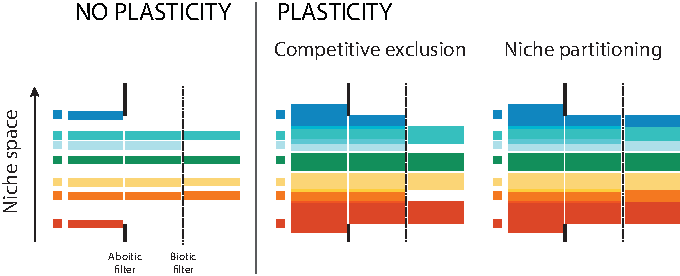
\includegraphics[width=1\linewidth]{./1_Introduction/graphics/filtering.pdf}
  \caption[Effect of plasticity of filters]{Phenotypic plasticity can affect filtering processes in diverse ways, making difficult the understanding of the role of plasticity in diversity maintenance.}
  \label{fig:plasticity_form}
\end{figure}

But plasticity responses not only depend on abiotic condition, but also on the neighbourhood that affects local environment \parencite{sultan_phenotypic_1995} at a fine scale. Because of plasticity, these interactions can even shift from competition to facilitation \parencite{callaway_phenotypic_2003}. A novel difficulty arises with the evidence that the identity of the competitor affects plastic response \parencite{callaway_phenotypic_2003, abakumova_plasticity_2016}, but it is likely that such interaction is related to traits and therefore impact on resource \parencite{callaway_phenotypic_2003}.

\paragraph{Functional diversity}

Species diversity often comes with functional diversity, however, phenotypic plasticity affect plant traits and is likely to affect functional diversity \parencite{albert_importance_2012}. Plasticity can lead to a convergence or a divergence of functional traits, decreasing or increasing functional diversity. In an experiment with legumes species \citet{roscher_contrasting_2015} observed these two phenomena on different types of traits, between monoculture and mixture. The convergence of canopy filling and vertical growth traits suggests that competition stresses the different species on light competition, leading to a reduction of working strategies along these dimensions. Whereas, relatively, the other aspects of plant development are less constraint, or species experience diverse and contrasting conditions in mixtures than in monocultures.\\




\textbf{Phenotypic plasticity is expected to increase the potential niche of species and reduce the filtering effect of abiotic conditions. However, the effect on biotic interaction makes no consensus and is likely to vary depending on the identity of the competitors, and the relative effect on trait differences. The balance between stabilizing niche differences and average fitness differences is crucial to determine the final impact on stable coexistence. The effects on functional diversity are also diverse but mainly depends on the plastic rules leading to convergence or divergence of traits.}
%But plasticity depends on neighbours: what does that change ?

%niche filling versus competitive exclusion: asymmetric gain and coexistence theory.

\subsection{Is productivity always improved?}

There is still debate on the effect of phenotypic plasticity of mechanisms driving species diversity, but is the question of the effect on productivity solved?

\paragraph{Stability}

Plasticity is a mechanism that emerges in a situation where the plants can increase their fitness in response to environmental conditions. This increase in fitness is often due to higher resource use or resource foraging efficiency and therefore better growth rate (observed in models \parencite{maire_plasticity_2013} and empirical studies \parencite{ hamann_evidence_2016}). This leads to higher individual productivity. It is especially true when resources are varying and these variations can be anticipated  \parencite{richter_phenotypic_2012}.

%Species able to deal with variations: stay relatively (more than without PP) when conditions don't match.

%pinus sylvestris gretter pl better in variable environment



\paragraph{Costs and limits}

However, has mentioned earlier, plasticity comes with inherent costs, related to the biological machinery needed to sense and process the signals and alter the phenotype. This costs, if the plant does not take advantage of the plasticity (no variability, in its niche) to increase (or maintain) growth rate will impact the productivity.

The unreliability of environmental cues is a limit of plasticity, and it can lead to maladaptive changes in phenotypes, but this is a marginal behaviour, and maladaptive plasticity is expected to be eliminated by an evolutionary process in fairly constant conditions. However, in the context of climate change, the reliability of these cues may decrease and leads to maladaptive responses. 

If unnecessary costs and unreliable cues can impact overall plant efficiency, adaptive plasticity can also hurt productivity while increasing fitness. Indeed, as evolutionary models and game theory predict, competition can lead to lower efficiency than optimum arrangement. Competition leading to lower resource availability, plastic species may have an aggressive plastic response leading to a stronger competitor but with less effective resource use.

%Competition behaviour may lead to suboptimum phenotypes.

%\paragraph{Diversity and productivity}
%
%Biodiversity - productivity
%
%Effects on
%
%Maintain different species: may change the productivity pattern. better at low prod, lower prod by introducing less productive species.


\subsection{Community identity shift}

The third main property of grassland communities is the \textemph{identity} of the dominant species (or average species if CWMs are considered). Phenotypic plasticity can impact community identity in two ways: (1) by shifting the identity of present species, (2) by altering the output of filtering processes in favour of different traits as presented in figure \ref{fig:identityshift}.


\begin{figure*}
    \classiccaptionstyle
\sidebysidecaption{0.5\textwidth}{0.4\textwidth}{%
    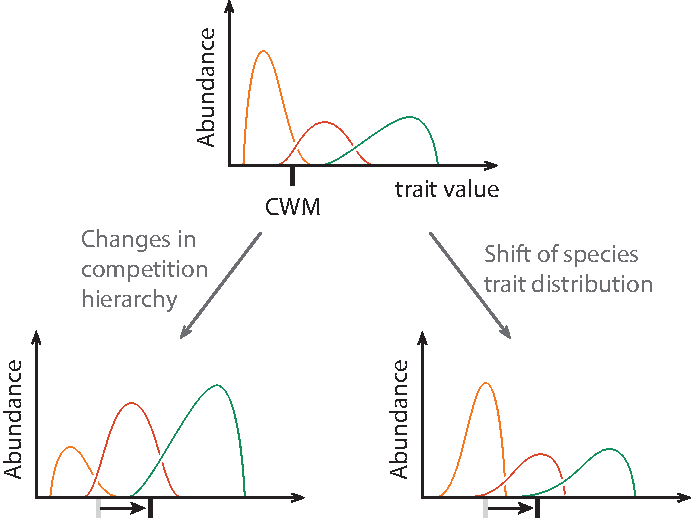
\includegraphics{./1_Introduction/graphics/identity_shift.pdf}
}{
  \caption[Identity shift]{Phenotypic plasticity effects on community identity. Phenotypic plasticity can modulate community-identity response to a change in conditions by two distinct but non exclusive mechanisms: altering the competitive hierarchy and species abundances (left) or shifting the individual species identity (right)\parencite{dwyer_specific_2014}.}
  \label{fig:identityshift}
  }
\end{figure*}

The first effect makes sense only in the context of a change in condition. Drought experiments in mountain grasslands show an intra-specific shift toward higher LDMC and lower SLA \parencite{jung_intraspecific_2014}. Other empirical studies show uncoupled response between above- and below-ground organs, shifting the strategy of the species \parencite{freschet_plasticity_2013}. A modelling experiment shows that the phenotypic plasticity is required to correctly model the dominance pattern along cutting frequency gradient \parencite{maire_plasticity_2013}, illustrating the second effect. \\

%selection of more or less resistant/digest/etc... species

%\textbf{Plasticity affect community identity by two independent mechanisms that might have contrasting outcomes. Both should be considered, therefore models should include both plastic response and population dynamics processes.}


\begin{figure}
    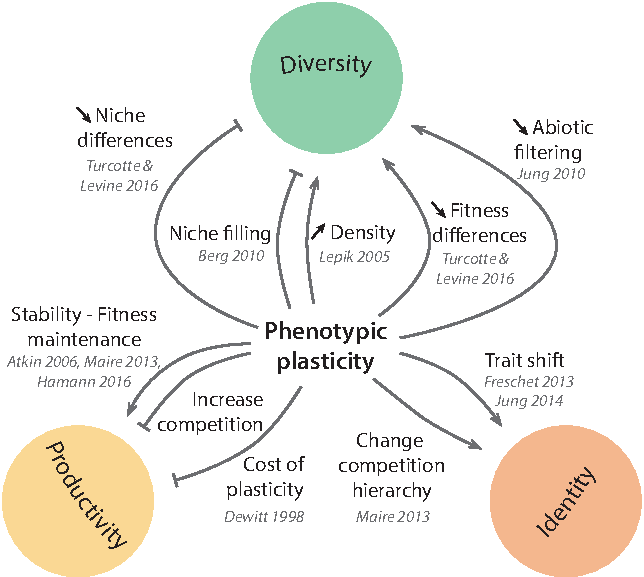
\includegraphics{./1_Introduction/graphics/effect_plasticity.pdf}
  \caption[Phenotypic plasticity effect on community properties]{Effect of phenotypic plasticity on the three main community properties. Phenotypic plasticity can impact these properties through multiple processes that may have contrasting effects. To determine the overall effect of plasticity on community response to changes in drivers (climate and land-use) we need to integrate all these effects.}
  \label{fig:plasticity-effect}
\end{figure}

%\subsection{Phenotypic plasticity effect on individuals and communities}

% section/chapter concluesion
%\paragraph{Contrasting effects}
%
%\paragraph{Interacting mechanisms}

% try to extract guidelines from the review of the literature.


% beginning on guidelines. Probably need a high level of modification
\textbf{Plasticity is a complex matter, both with a growth process that alters strategies and a strategy itself. New simulations tools for understanding community dynamics should try to both include multiple coexistence mechanisms and plant strategies. They should focus on the individual level mechanisms of competition, growth, and survival and observe the emerging patterns at the scale of the community. This can only be achieved in a constrained high dimensional strategy space based on physical and biological trade-offs. Individual-level modelling allows the integration of multiple sources of intra-specific variability: genetic diversity and phenotypic plasticity. The phenotypic plasticity being driven by the perception of the environment, it cannot be simply described by normal random distribution but should be build on a coherent framework allying physiological, morphological and evolutionary constraints. This focus is particularly important considering both the lack of understanding of this phenomenon and the consequences for plant communities.  }


